%Documento principal do latex para uso no TCC da Univás.

\documentclass[a4paper, 12pt, chapter=TITLE, oneside, english, brazil]{abntex2}

\usepackage{styles/CodeStyle}      %Formatação de códigos e listagens
\usepackage{styles/EventFlowStyle} %Estilo para o quadro de fluxo de eventos
\usepackage{styles/NuapaStyle}     %Estilo exigido pela Univás
\usepackage{lscape}

%Início do documento
\begin{document}
%\overfullrule=100mm
\pretextual %Início dos Elementos Pré-Textuais


\makeatletter
\renewcommand{\imprimircapa}{%
\begin{capa}%
\begin{center}%
	\begin{SingleSpacing}
	{\ABNTEXchapterfont\large\MakeUppercase\imprimirautor}\\
	\end{SingleSpacing}
  
  \vspace*{\fill}%
  \vspace*{\fill}%
  \vspace*{\fill}%
  {\ABNTEXchapterfont\bfseries\Large\MakeUppercase\imprimirtitulo}\\
  \vspace*{\fill}%
  {\color{white}%
\abntex@ifnotempty{\imprimirpreambulo}{%
  \hspace{.45\textwidth}
  \begin{minipage}{.5\textwidth}
    \SingleSpacing
    \imprimirpreambulo
  \vspace{.1\textwidth}\\%
  {\imprimirorientadorRotulo:~\imprimirorientador}
  \abntex@ifnotempty{\imprimircoorientador}{%
    \hspace{.45\textwidth}
    {\large\imprimircoorientadorRotulo~\imprimircoorientador}%
  }%
  \end{minipage}%
}%
\color{black}}%
  \vspace*{\fill}\\%
  \begin{SingleSpacing}
  	
  {\ABNTEXchapterfont\large\bfseries\MakeUppercase\imprimirinstituicao}\\
  {\large\bfseries\MakeUppercase\imprimirlocal}\\
  {\large\bfseries\MakeUppercase\imprimirdata}
  \end{SingleSpacing}
\end{center}
\end{capa}
}
\makeatother

\imprimircapa

% folha de rosto s
%\folhaderostoname{Folha de rosto}
%http://code.google.com/p/abntex2/wiki/ComoCustomizar

\makeatletter
\renewcommand{\folhaderostocontent}{
\begin{center}%
	\begin{SingleSpacing}
		{\ABNTEXchapterfont\large\MakeUppercase\imprimirautor}\\
	\end{SingleSpacing}
  
  \vspace*{\fill}%
  \vspace*{\fill}%
  \vspace*{\fill}%
  
  {\ABNTEXchapterfont\bfseries\Large\MakeUppercase\imprimirtitulo}\\
  \vspace*{\fill}%
\abntex@ifnotempty{\imprimirpreambulo}{%
  \hspace{.45\textwidth}
  \begin{minipage}{.5\textwidth}
    \SingleSpacing
    \imprimirpreambulo
  \vspace{.1\textwidth}\\%
  {\imprimirorientadorRotulo:~\imprimirorientador}
  \abntex@ifnotempty{\imprimircoorientador}{%
    \hspace{.45\textwidth}
    {\large\imprimircoorientadorRotulo~:\imprimircoorientador}%
  }%
  \end{minipage}%
}%
  \vspace*{\fill}\\%
  
  \begin{SingleSpacing}
  	{\ABNTEXchapterfont\large\bfseries\MakeUppercase\imprimirinstituicao}\\
  	{\large\bfseries\MakeUppercase\imprimirlocal}\\
  	{\large\bfseries\MakeUppercase\imprimirdata}
  \end{SingleSpacing}
  
\end{center}
}%end of folhaderostocontent
\makeatother

\imprimirfolhaderosto*{}
%\begin{fichacatalografica}
\begin{normalsize}
  \vspace*{\fill}
  % Posição vertical
%  \hrule
  % Linha horizontal
  \begin{center}
  \fbox{
    % Minipage Centralizado
    \begin{minipage}[c]{12.5cm} % Largura
      \vspace{0.7cm}%
      \hspace{0.8cm} \imprimirAutorCitacao ~\\%
      
      \hspace{0.8cm} \imprimirtitulo ~/ \imprimirAutorUm , \imprimirAutorDois ~-- \imprimirlocal: Univás, \imprimirdata. %
      
      \hspace{0.8cm} \pageref{LastPage} f. : il.~\\%
      
      \hspace{0.8cm} \imprimirtipotrabalho~--~\imprimirinstituicao , Univás, \imprimircurso. % 
      
      \hspace{0.8cm} \imprimirorientadorRotulo: ~\imprimirorientador ~\\%

      \hspace{0.8cm} 1. \imprimirPalavraChaveUm. 2. \imprimirPalavraChaveDois. 3. \imprimirPalavraChaveTres. ~ \\%
    \end{minipage}
    }
  \end{center}
\end{normalsize}
\end{fichacatalografica}
\newpage
%\setlength{\ABNTEXsignwidth}{10cm}

\begin{folhadeaprovacao}
  \begin{center}
    {\ABNTEXchapterfont\large\MakeUppercase\imprimirautor}
    \vspace*{\fill}
    \vspace*{\fill}
    \vspace*{\fill}
    \par
    {\ABNTEXchapterfont\bfseries\Large\MakeUppercase\imprimirtitulo}
    \vspace*{\fill}
  \end{center}
  Trabalho de conclusão de curso defendido e aprovado em \imprimirDataDaAprovacao ~pela banca examinadora constituída pelos professores:

  ~\newline
  \begin{flushleft}
  \assinatura*{\imprimirorientador \\ \imprimirorientadorRotulo }
  \assinatura*{\imprimirAvaliadorUm \\ \imprimirAvaliadorLabelUm }
  \assinatura*{\imprimirAvaliadorDois \\ \imprimirAvaliadorLabelDois}
  \end{flushleft}
  \vspace*{\fill}
  \vspace*{\fill}
\end{folhadeaprovacao}

\begin{dedicatoria}
	\vspace*{\fill}
	
	De \imprimirAutorUm.
	\newline
	%início da dedicatória do autor um
	Dedico este trabalho primeiramente a Deus, que me concedeu saúde e motivação
	para lutar e conquistar meus objetivos. Aos meus pais Mauro Nunes da Silva e
	Vera Lúcia da Silva, que tanto se dedicaram para que eu pudesse estudar e
	realizar meus sonhos. Por fim, dedico a todas as pessoas que, de um modo ou
	outro, contribuíram pelo meu crescimento ético, pessoal e profissional.
	
	\vspace*{\fill}
	De \imprimirAutorDois.
	\newline
	%início da dedicatória do autor dois
	\par Dedico este trabalho, primeiramente, a Deus e sua Santíssima Mãe que me
	deram força e saúde para vencer esta luta, considerada por mim, uma
	batalha, independente do resultado. Dedico também aos meus pais Joaquim
	Coutinho de Rezende e Maria José Cirino Rezende, que se dedicaram ao extremo,
	se privando muitas vezes de coisas necessárias, para meu conforto e para que eu
	pudesse progredir como pessoa e como profissional. Dedico ao meu irmão Djalma
	Lúcio Rezende, por ser meu amigo e pela sua ajuda valiosa. Dedico a minha vó
	Maria do Carmo Cirino por ser para mim um exemplo de paciência e humildade,
	pois posso afirmar com certeza que foram suas orações que me mantiveram de pé.
	E por fim, dedico a todas as pessoas do meu dia-a-dia, que passaram por essa
	batalha comigo.

\end{dedicatoria}

\begin{agradecimentos}

De \imprimirAutorUm
\newline
%início do agradecimento do autor um
\par Agradeço \ldots

\vspace*{\fill}
De \imprimirAutorDois
\newline
%início do agradecimento do autor dois
\par Agradeço \ldots

\end{agradecimentos}





%\begin{epigrafe}
\vspace*{\fill}
\begin{flushright}
\textit{‘‘Complicar é simples, \\
simplificar que é complicado.\\
(Paulo Sérgio dos Santos)}
\end{flushright}
\end{epigrafe}

% --- resumo em português ---

\begin{OnehalfSpacing} 

%\noindent \imprimirAutorCitacaoMaiuscula. {\bfseries\imprimirtitulo}.
% {\imprimirdata}.  Monografia -- Curso de {\MakeUppercase\imprimircurso},
% {\imprimirinstituicao}, {\imprimirlocal}, {\imprimirdata}.

\vspace{\onelineskip}
\vspace{\onelineskip}
\vspace{\onelineskip}
\vspace{\onelineskip}

\begin{resumo}
~\\
%início do texto do resumo
\noindent Atualmente, existe uma grande quantidade de tecnologias disponíveis
no mercado e sabe-se também, que com a popularização dos \textit{smartphones} e
\textit{tablet} tornou-se comum utilizar dispositivos móveis para receber
informações em tempo real. Neste contexto, nesta pesquisa foi desenvolvido um
\textit{web service} para disponibilizar as informações de discentes da Univás
através de serviços. Também foi criado um aplicativo na plataforma Android que
consome o serviço do \textit{web service}. O \textit{app} permite aos alunos da
Universidade do Vale do Sapucaí consultarem suas informações acadêmicas como
notas, faltas e provas agendadas do semestre corrente. No momento em que um
professor lançar um evento, o servidor transmite a mensagem para a API Google
Cloud Messaging (GCM) que se responsabiliza em entregar os dados para o
aplicativo Android. Este trabalho enquadra-se no tipo de pesquisa aplicada,
pois foi desenvolvido um produto real com propósito de resolver um problema
especifico. A plataforma Android foi escolhida pelo seu destaque no mercado.

%fim do texto do resumo
\vspace{\onelineskip}
\vspace*{\fill}
\noindent \textbf{Palavras-chave}: \imprimirPalavraChaveUm. \imprimirPalavraChaveDois. \imprimirPalavraChaveTres.
\vspace{\onelineskip}
\end{resumo}

\end{OnehalfSpacing}

% --- resumo em inglês ---

\begin{OnehalfSpacing} 

\noindent \imprimirAutorCitacaoMaiuscula. {\bfseries\imprimirtitulo}.
 {\imprimirdata}.  Monografia -- Curso de {\MakeUppercase\imprimircurso},
 {\imprimirinstituicao}, {\imprimirlocal}, {\imprimirdata}.

\vspace{\onelineskip}
\vspace{\onelineskip}
\vspace{\onelineskip}
\vspace{\onelineskip}

\begin{resumo}[Abstract]%
\begin{otherlanguage*}{english}%
\textit{
%início do texto do abstract
\noindent Currently, there is a lot of technology available in the market and it
is also known that with the popularization of smartphones and tablets has
become common to use of mobile devices to receive information in real time. In
this context, in the research was developed a web service to provide
information from Univas by this service. It was also created an application on
the Android platform that consumes the use of web service. The app allows
students at the University of Vale do Sapucai  consult their academic
information such as grades, absences and tests of the current semester. When a
teacher launch an event, the server transmits the message to API Google Cloud
Messaging (GCM) that is responsible for the data delivery to the Android
application. This work  fits in the type of applied research because it was
developed a real product with purpose to solve a specific problem. The Android
platform was chosen for its  prominent position in the market.
%fim do texto do abstract
}

\vspace{\onelineskip}
\vspace*{\fill}
\noindent \textbf{Key words}: \imprimirKeyWordOne. \imprimirKeyWordTwo. \imprimirKeyWordThree.
\end{otherlanguage*}
\vspace{\onelineskip}
\end{resumo}

\end{OnehalfSpacing}

%Lista de Figuras
\pdfbookmark[0]{\listfigurename}{lof}
\listoffigures*
\cleardoublepage

%Lista de siglas
%ver http://marc.info/?l=tex-br&m=110566665520790 para colocar em ordem alfabética.

\begin{SingleSpace}

	\begin{siglas}
		
		\item[ACID] Atomicidade, consistência, isolamento e Durabilidade
		
		\item[API] \textit{Application Programming Interface}
		
		\item[GCM] \textit{Google Cloud Messaging}

		\item[HTTP] \textit{HyperText Transfer Protocol}

		\item[ID] \textit{Identity}
		
		\item[IDE] \textit{Integrated Development Environment}
		
		\item[I/O] \textit{Input/Output}
		
		\item[JVM] \textit{Java Virtual Machine} 
		
		\item[JSON] \textit{JavaScript Object Notation}

		\item[KB]	\textit{kilobyte}
		
		\item[REST] \textit{Representational State Transfer}
		
		\item[SGBD] Sistema de Gerenciamento de Banco de Dados
				
		\item[SSL] \textit{Secure Socket Layer}
		
		\item[SQL] \textit{Structured Query Language}
		
		\item[UNIVAS] Universidade do Vale do Sapucaí
				
		\item[URL] \textit{Universal Resource Locator}
		
		\item[XML] \textit{Extensible Markup Language}
	
	\end{siglas}

\end{SingleSpace}


% Lista de Quadros
\pdfbookmark[0]{\listofquadrosname}{loq}
\listofquadros*
\cleardoublepage

%Lista de Tabelas
\pdfbookmark[0]{\listtablename}{lot}
\listoftables*
\cleardoublepage


%Sumário
%ver esse link para configuração de fonte: http://tex.stackexchange.com/questions/83377/how-to-change-chapter-font-style-in-the-middle-of-the-table-of-the-contents
\pdfbookmark[0]{\contentsname}{toc}
\begin{SingleSpace} 
\tableofcontents*
\end{SingleSpace}
\cleardoublepage


\textual %Início dos Elementos Textuais

%\chapter*{Introdução}
%\begin{center}
  \vspace{1.2em}
  \textbf{\large INTRODUÇÃO}
  \vspace{2.9em}
%\end{center}
\thispagestyle{empty}

\addcontentsline{toc}{chapter}{INTRODUÇÃO}
\stepcounter{chapter} %incrementa o número do capítulo

	\par Atualmente, com os avanços tecnológicos, as pessoas estão cada vez mais
conectadas e procuram soluções para seus problemas, que as ajudem de forma
móvel, rápida e fácil. Segundo \citeonline{lacheta2013}, tanto as empresas
quantos os desenvolvedores buscam plataformas modernas e ágeis para a criação de
aplicações. Esse fato contruibuiu consideravelmente para o crescimento das
plataformas móveis de comunicação.

	\par Uma das áreas que mais se expandiu nos últimos anos é a de telefonia
móvel. \\\citeonline[p.1]{monteiro2012} afirma que “os telefones celulares
foram evoluindo, ganhando cada vez mais recursos e se tornando um item quase
indispensável na vida das pessoas”. Essa evolução no \textit{hardware}
possibilitou o crescimento, mobilidade e portabilidade do \textit{software}.

	\par Muito das coisas que antes eram feitas somente em computadores
\textit{desktops} já podem ser realizadas nos celulares, como transferências
bancarias, localização de taxi, conversas com amigos, entretenimento com jogos
e vídeos, entre outros.

	\par De acordo com \citeonline{monteiro2012}, a plataforma \textit{Android} se
destaca no mercado devido ao grande número de aparelhos espalhados pelo mundo e
pela facilidade que provêem aos desenvolvedores.

	\par A plataforma \textit{Android} foi utilizada para o desenvolvimento de
vários trabalhos de conclusão de curso como por exemplo \citeonline{mendes2011}
que criou um aplicativo para que as bandas musicais pudessem ter mais interação com
seus fãs. \citeonline{oglio2013} do Centro Universitário Univates, criou um
sistema que permite o acesso ao portal virtual da sua faculdade.

	\par Pelas facilidades que \textit{smartphones} provêem para conseguir
informações rápidas a qualquer hora e local, pensa-se em criar um utilitário
que possibilite aos usuários consultarem as suas notas, presenças e provas
agendadas no portal do aluno.

\chapter{OBJETIVOS}
	
	\par Neste capítulo serão descritos os objetivos a serem atingidos com a
presente pesquisa.
	
\section{Objetivo Geral}

	\par Desenvolver um aplicativo para a plataforma \textit{Android}, que permita
aos alunos da Universidade do Vale do Sapucaí consultarem suas notas, presenças
e provas agendas pelo seu \textit{smartphone}.

\section{Objetivos Específicos}

	\par A seguir serão descritos os objetivos específicos para construção do
\textit{software} proposto no objetivo geral dessa pesquisa. São eles:
	
	\begin{itemize}
	  \item Levantar requisitos do \textit{software} proposto de acordo com as
	  necessidades dos alunos.
	  \item Planejar o projeto.
	  \item Desenvolver o aplicativo para celular.
	  \item Desenvolver um \textit{web service} que fará a comunicação entre o
	  aplicativo e o servidor da universidade.
	  \item Realizar testes.
	\end{itemize}
	
	\par Com esses passos espera-se fazer um \textit{software} eficaz que auxiliará
no dia-a-dia dos alunos.

\chapter{JUSTIFICATIVAS}

	\par A escolha por fazer um aplicativo se deu pela necessidade em acessar o
portal do aluno para ter informações referente às disciplinas. Com o projeto 
espera-se contribuir socialmente facilitando o acesso dos usuários às suas notas, 
provas agendadas e faltas.

	\par O trabalho também auxiliará os alunos do curso de Sistemas de Informação
que necessitarem saber como se desenvolve um aplicativo na plataforma
\textit{Android} ou implementar mais funcionalidades nesse projeto.

	\par A plataforma \textit{Android} será utilizada devido a grande popularidade
do sistema operacional.

	\par Visando facilitar as pesquisas aos conteúdos publicados no portal do
alunos, quer-se desenvolver um App\footnote{Abreviação para a palavra \textit{Application}},
pela qual os discentes os terão facilmente.

\chapter{QUADRO TEÓRICO}

	\par Neste capítulo serão descritos os principais conceitos e características
das tecnologias utilizadas para o desenvolvimento dos \textit{softwares}
propostos nos objetivos deste trabalho.

%java
\section{\textit{Java}}

	\par Conforme \citeonline{deitel2010}, \textit{Java} é uma linguagem de
programação orientada objetos, baseada na linguagem C++, desenvolvida pela
empresa \textit{Sun Microsystem} no ano de 1995, por uma equipe sob liderança
de James Gosling.

	\par Segundo \citeonline{caelum3}, para executar as aplicações, o
\textit{Java} utiliza uma máquina virtual denominada JVM\footnote{JVM - Java
Virtual Machine}, que liberta os softwares de ficarem presos a um único sistema
operacional, uma vez que o programa conversa diretamente com a JMV e fica por
conta dela traduzir os \textit{bytecodes} gerados pelo compilador para
linguagem de máquina.

	\par De acordo com \citeonline{java}, o \textit{Java} está presente em mais de
um bilhão de dispositivos como celulares, computadores, consoles de
\textit{games} e pode ser considerado, seguro, rápido e confiável.

	\par Hoje, com a acenção do \textit{Android}, a tendência é aumentar cada vez
mais o desenvolvimento em \textit{Java}, uma vez que os aplicativos Android são
desenvolvidos nessa linguagem. Nessa pesquisa a linguagem de programação
\textit{Java} será utilizado no desenvolvimento tanto do aplicativo quanto do
\textit{web service}.
%android
%\section{Android}

	\par Segundo \citeonline{monteiro2012}, Android é um sistema operacional
baseado em Linux, que utiliza a linguagem de programação Java para o
desenvolvimento de seus aplicativos. Criado especialmente para dispositivos
móveis, começou a ser desenvolvido no ano de 2003 pela então empresa Android
Inc, que em 2005 foi agregada ao Google. A partir de 2007 o projeto Android
uniu-se a Open Handset Alliance, uma associação de empresas de
softwares, hardwares e telecomunicações, que tem por finalidade desenvolver uma
plataforma para dispositivos móveis que seja completa, aberta e gratuita.

	\par \citeonline{krazit2009} afirma que o sistema pode rodar em equipamentos
de diversos fabricantes, evitando assim ficar limitado a poucos dispositivos.
Conforme informações do site \citeonline{android1}, hoje em dia existe mais de
um bilhão de aparelhos espalhados pelo mundo com esse sistema operacional.

	\par De acordo com \citeonline{monteiro2012}, as aplicações são executadas em
uma máquina virtual Java denominada Dalvik. Cada aplicativo, usa uma instância
dessa máquina virtual, tornando-o assim mais seguro. Por outro lado, os
softwares só podem acessar os recursos do dispositivo, como uma lista de
contatos, caso seja formalmente aceito pelo usuário nos termos de uso, ao
instalá-lo.

	\par As configurações de uma aplicação na plataforma Android ficam salvas em um
arquivo XML\footnote{XML - \textit{Extensible Markup Language}.} denominado
\texttt{AndroidManifest.xml}, que se localiza na pasta raiz do projeto. Para
\citeonline{lecheta2010}, as informações devem estar entre \textit{tags}
correspondentes ao recurso.

	\par \citeonline{lecheta2010} diz que as Intents são recursos tão importantes
que podem ser consideradas como o coração do Android e que estão presentes em
todas as aplicações.	De acordo com \citeonline[p.29]{k192012}, "Intents são
objetos responsáveis por passar informações, como se fossem mensagens, para os
principais componentes da API do Android, como as Activities, Services e
BroadCast Receivers". \citeonline{monteiro2012} diz que as Intents são criadas
quando se tem a intenção de realizar algo como por exemplo compartilhar uma
imagem, utilizando os app's já existentes no dispositivo. Existem dois tipos de
Intents:
	
	\begin{itemize}
	  
	  \item Intents implícitas: quando não é informada qual activity deve ser
	  chamada, ficando assim por conta do sistema operacional verificar qual é a
	  melhor opção.
	  
	  \item Intents explícitas: quando é informada qual activity deve ser chamada.
	  Usada normalmente para chamar \textit{activities} da mesma aplicação.
	  
	\end{itemize}
	
	\par Segundo \citeonline{k192012}, uma aplicação Android pode ser construída
com quatro tipos de componentes: Activity, Services, Content Providers e
Broadcast Receivers.

	\par As \textit{activities} são as telas com interface gráfica, que permitem
interações com os usuários. De acordo com \citeonline{lacheta2013}, cada
\textit{activity} tem um ciclo de vida, uma vez que ela pode estar sendo
executada, estar em segundo plano ou totalmente destruída.

	\par Toda vez que é iniciada uma activity, ela vai para o topo de uma pilha
denominada \textit{activity stack}. O bom entendimento de seu ciclo de vida é
importante, pois quando uma aplicação é interrompida, é possível salvar as
informações ou ao menos voltar ao estágio a qual o usuário se encontrava. Na
Figura \ref{fig:qt1} é demonstrado o ciclo de vida de uma \textit{activity}.

	\begin{figure}[h!]
		\centerline{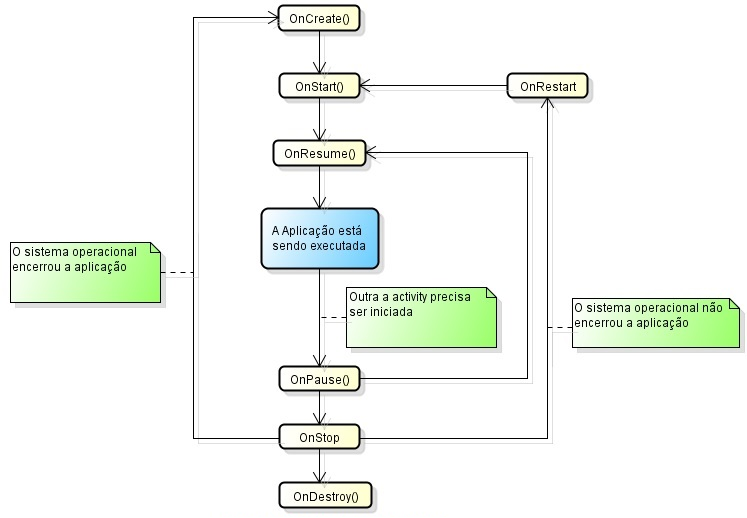
\includegraphics[scale=0.8]{./imagens/1_q_teorico/qt1.png}}
		\caption[Ciclo de Vida de uma Activity]{Ciclo de Vida de uma
		Activity.
		 \textbf{Fonte:}\citeonline{lecheta2010}}
		\label{fig:qt1}
	\end{figure}

	\par Para que se possa entender melhor, imagina-se o seguinte cenário: um
usuário entra no aplicativo de notas da Univás. Para que a \textit{activity}
seja criada, é chamado o método \texttt{onCreate()}, logo após é executado o
método \texttt{onStart()} e ao finalizar do ciclo anterior é chamado o
\texttt{onResume()}, só a partir de então, a \textit{activity} é visualizada
pelo discente. Contudo, durante a navegação, o aluno recebe uma ligação, então
nessa hora o sistema operacional chama o método \texttt{onPause()} para
interromper a aplicação e abrir uma outra \textit{activity} para que o usuário
possa atender a chamada telefônica. É possível, nesse método, salvar
informações que o usuário está utilizando. Ao concluir o método de pausa, é
executado o método \texttt{onStop()}, a partir de agora a \textit{activity} da
Univás não será mais visível ao usuário.

 	\par Ao encerrar a ligação, há dois caminhos possíveis de se percorrer, o
primeiro, seria o caso do sistema operacional encerrar completamente a
aplicação, por necessidade de liberar espaço em memória. Para destrui-la é
chamado o método \texttt{onDestroy()}. Dessa forma, para executar o aplicativo
da Univás será necessário chamar o método \texttt{onCreate()} novamente
seguindo o ciclo normal. Porém se não for encerrada completamente, ao findar a
ligação será executado o método \texttt{onRestart()} e voltar para a
\textit{activity} ao qual o usuário se encontrava.

	\par No arquivo \texttt{AndroidManifest.xml} as \textit{activities} devem estar
entre as tags \texttt{<activity> </activity>} e a \textit{activity} principal,
ou seja, pela qual será iniciada a aplicação deve conter a \textit{tag}
\texttt{<intent-filter>} além de \texttt{<action
android:name="android.intent.action.MAIN"/>} indicando que essa atividade
deverá ser chamada ao iniciar a aplicação e \texttt{<category
android:\\name="android.intent.category.LAUNCHER"/>} que implica que esse
APP ficará disponível junto aos outros aplicativos no dispositivo.
Na figura \ref{fig:qt2} é apresentado o código do arquivo
\texttt{AndroidManifest.xml}. Nela, pode-se ver o nome da classe que será
iniciada e no atributo \textit{label} o nome que aparecerá na tela para o
usuário.
	
	\begin{figure}[h!]
		\begin{lstlisting}[style=custom_XML]
		  <activity
	            android:name=".MainActivity"
	            android:label="@string/app_name" >
	            <intent-filter>
	                <action android:name="android.intent.action.MAIN" />
	                <category android:name="android.intent.category.LAUNCHER" />
	            </intent-filter>
	      </activity>
		\end{lstlisting}
		\caption[Código do arquivo
		AndroidManifest.xml indicando qual activity deve ser executada quando a
		aplicação iniciar]{Código do arquivo \texttt{AndroidManifest.xml} indicando
		qual \textit{activity} deve ser executada quando a aplicação iniciar.
		 \textbf{Fonte:}Elaborado pelos autores}
		\label{fig:qt2}
	\end{figure}
	
	\par A \textit{Activity} a ser utilizada para iniciar a aplicação é uma
\texttt{Navigation Drawer}, que segundo o site \citeonline{android2015}, ela exibe
do lado esquerdo as principais funções do software, semelhante a um
menu, que fica normalmente escondida aparecendo apenas quando clicado no canto
superior esquerdo. 

	\par Segundo \citeonline{lecheta2010}, a classe \texttt{Service} existe com o intuito
de executar processos que levarão um tempo indeterminado para serem executados
e que normalmente consomem um alto nível de memória e processamento. Esses
processos são executados em segundo plano enquanto o cliente realiza outra
tarefa. Assim um usuário pode navegar na internet enquanto é feito um
\textit{download}. O serviço é geralmente iniciado pelo \texttt{Broadcast Receiver} e
quem o gerencia é o sistema operacional que só o finalizará ao concluir a
tarefa, salvo quando o espaço em memória é insuficiente.

	\par Para \citeonline{lecheta2010}, um \texttt{Content Provider} provê conteúdos de
forma pública para todas as aplicações, possibilitando aos aplicativos consultar,
salvar, deletar e alterar informações no \textit{smartphone}. Assim afirma
\citeonline[p.413]{lecheta2010} “o Android tem uma série de provedores de
conteúdo nativos, como, por exemplo, consultar contatos da agenda, visualizar
os arquivos, imagens e vídeos disponíveis no celular”. Portanto, um contato
pode ser salvo na agenda de contatos do dispositivo por um aplicativo e
alterado por outro.

	\par Para \citeonline{monteiro2012}, o \texttt{Broadcast Receiver},
é um componente do Android responsável por responder a eventos do sistema.
Ele não possui interface gráfica e normalmente interage com os usuários através
de notificações.

	\par Outra ferramenta importante e muito utilizada do Android é a Notificação.
Segundo \citeonline{phillips2013} quando uma aplicação está sendo
executada em segundo plano e necessita comunicar-se com o usuário, o aplicativo
cria uma notificação. Normalmente as notificações aparecem na barra superior, o
qual pode ser acessado arrastando para baixo a partir da parte superior da
tela. Assim que o usuário clica na notificação ela cria uma \textit{activity}
para abrir  aplicação em questão.

	\par O Android traz embarcado em sua plataforma o banco de dados
\texttt{SQLite}, que armazena tabelas, \textit{views}, índices,
\textit{triggers} em apenas um arquivo em disco. Somente é possível acessa-lo
pela aplicação a qual o criou e, é deletado caso o aplicativo seja removido.

	\par Na seção abaixo serão descritos os elementos gráficos presentes no
Android.

	
%androidstudio
\section{Android Studio}

	\par Umas das ferramentas mais utilizadas para o desenvolvimento em Android é o
\textit{Eclipse IDE}, contudo a Google criou um \textit{software} especialmente
para esse ambiente, chamado \textit{Android Studio}. Segundo
\citeonline{gusmao2014}, \textit{Android Studio} é uma IDE baseado no ItelliJ
\textit{Idea} e foi apresentado na conferência para desenvolvedores I/O de 2013.

	\par De acordo com \citeonline{hohensee2013}, o \textit{Android Studio} tem um
sistema de construção baseado em \textit{Gradle}, que permite aplicar
diferentes configurações no código quando há necessidade de criar mais de uma
versão, como por exemplo, um \textit{software} que terá uma versão gratuita e
outra paga, melhorando a reutilização do código. Com o \textit{Gradle} também é
possível fazer os \textit{downloads} de todas as dependências de uma forma
automática sem a necessidade de importar bibliotecas manualmente.

	\par \citeonline{hohensee2013} afirma que o \textit{Android Studio} é um editor
de código poderoso, pois tem como característica a edição inteligente, que ao
digitar já completa as palavras reservadas do \textit{Android} e fornece uma
organização do código mais legível.

	\par Segundo \citeonline{android2}, a IDE tem suporte para a edição de
interface, o que possibilita ao desenvolvedor arrastar os componentes que
deseja. Ao testar o aplicativo, ela permite o monitoramento do consumo de
memória e de processador por parte do utilitário.

	\par \citeonline{gusmao2014} diz que a plataforma tem uma ótima integração com
o \textit{GitHub} e está disponível para \textit{Windows}, \textit{Mac} e
\textit{Linux}. Além disso os programadores terão disponíveis uma versão
estável e mais três versões que serão em teste, chamadas de \textit{Beta},
\textit{Dev} e \textit{Canary}.

	\par Devido a fácil usabilidade e por ser a IDE oficial para o desenvolvimento
\textit{Android}, escolheu-se esse ambiente para a construção do aplicativo.
%webservices
%\section{\textit{Web Services}}
	
	\par Nos tempos atuais, com o grande fluxo de informação que percorre pela
internet, é necessário um nível muito alto de integração entre as diversas
plataformas, tecnologias e sistemas. Como uma provável solução para esse ponto,
já existem as tecnologias de sistemas distribuídos. Porém essas tecnologias
sofrem demasiadamente com o alto acoplamento de seus componentes e também com a
grande dependência de uma plataforma para que possam funcionar. Com intuito de
solucionar estes problemas e proporcionar alta transparência entre as várias
plataformas, foram criados as tecnologias \textit{web services}.
	
	
	\par De acordo com \citeonline[s.p]{erl2015}:
	\begin{citacao}
		No ano de 2000, a W3C (\textit{World Wide Web Consortium}) aceitou a submissão
		do \textit{Simple Object Access Protocol} (SOAP). Este formato de mensagem
		baseado em XML estabeleceu uma estrutura de transmissão para comunicação entre
		aplicações (ou entre serviços) via HTTP\footnote{HTTP - \textit{HyperText
		Transfer Protocol}}. Sendo uma tecnologia não amarrada a fornecedor, o SOAP
		disponibilizou uma alternativa atrativa em relação aos protocolos
		proprietários tradicionais, tais como CORBA e DCOM.
	\end{citacao}
	
	\par De acordo com \citeonline{duraes2005}, \textit{web service} é um
componente que tem por finalidade integrar serviços distintos. O que faz com
que ele se torne melhor que seus concorrentes é a padronização do XML
(\textit{Extensible Markup Language}) para as trocas de informações. A
aplicação consegue conversar com o servidor através do  WSDL que é o documento
que contém a estrutura do \textit{web service}.
	
	\par Segundo \citeonline{coulouris2013}, “Um serviço \textit{web} (\textit{web
service}) fornece uma interface de serviço que permite aos clientes interagirem
com servidores de uma maneira mais geral do que acontece com os navegadores
\textit{web}”. Ainda de acordo com \citeonline{coulouris2013}, os clientes (que
podem ser desde um navegador até mesmo outro sistema) acessam serviços 
\textit{web} fazendo uso de requisições e respostas formatadas em XML e sendo
transmitidos pelo uso do protocolo HTTP. O uso dessas tecnologias tende a
facilitar a comunicação entre as diversas plataformas, e atende de uma
melhor forma que as tecnologias existentes. Porém, para que haja uma
interação transparente e eficaz, entre as diversas plataformas, é necessário uma
infraestrutura um pouco mais complexa para integrar todas essas tecnologias.
Essa infraestrutura é composta pelas tecnologias já citadas e por outros
componentes essenciais para disponibilização de serviços \textit{web}, como
mostra a Figura \ref{fig:ws}.

\begin{figure}[h!]
	\centerline{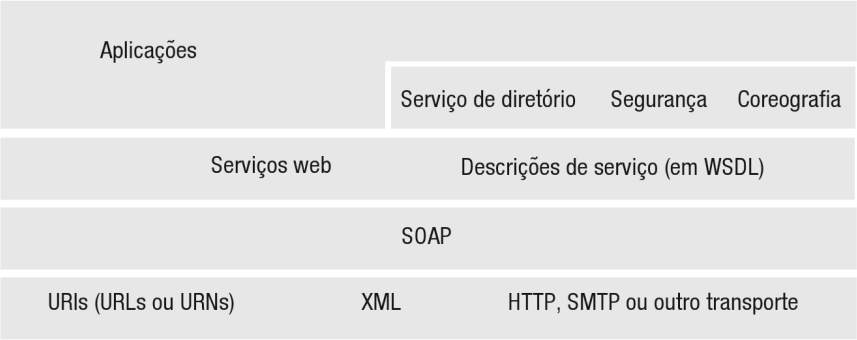
\includegraphics[scale=0.7]{./imagens/1_q_teorico/qt2.png}}
	\caption[Infraestrutura e componentes dos serviços
		\textit{web}. ]{Infraestrutura e componentes dos serviços
		\textit{web}. \textbf{Fonte:}\citeonline{coulouris2013}}
	\label{fig:ws}
\end{figure}
	
	\par Os \textit{web services} geralmente fazem uso do protocolo SOAP, para
estruturar e encapsular as mensagens trocadas. De acordo com
\citeonline[p.381]{coulouris2013}, "o protocolo SOAP é projetado para permitir
tanto interação cliente-servidor de forma assíncrona pela Internet". Segundo
\citeonline[p.27]{sampaio2006}, "o SOAP foi criado inicialmente, para
possibilitar a invocação remota de métodos através da internet".

	\par As mensagens SOAP possuem um elemento envelope, que de acordo com
\citeonline[p.19]{saudate2013}, "é puramente um \textit{container} para os
elementos \textit{Header} e \textit{Body}". O elemento \textit{header}
transporta metadados relativos à requisição tais como autenticação, endereço de
retorno da mensagem, etc. Já o elemento \textit{body} carrega o corpo da
requisição, que nada mais é do que o nome da operação e paramêtros referentes à
mesma. É válido lembrar que todas requisições são trocadas usando SOAP, e usam
o XML como formato oficial. 
%Na Figura \ref{fig:qt3} está representado o esquema do Envelope SOAP.
	
%\begin{figure}[h!]
%	\centerline{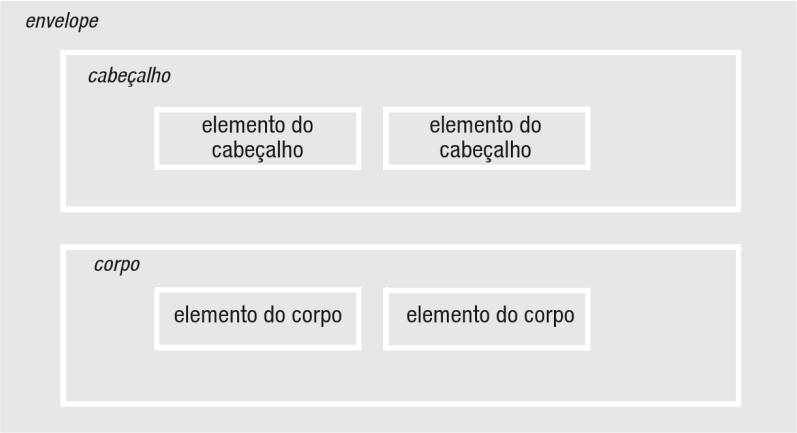
\includegraphics[scale=0.6]{./imagens/1_q_teorico/qt3.png}}
%	\caption[Esquema de envelope SOAP. ]{Esquema de envelope SOAP. 
%	 \textbf{Fonte:}\citeonline{coulouris2013}}
%	\label{fig:qt3}
%\end{figure}

	\par Os \textit{web services}, além de fornecerem uma padronização de
comunicação entre as várias tecnologias existentes, proveem transparência na
troca de informações. Isso contribui para que as novas aplicações consigam se
comunicar com aplicações mais antigas ou aplicações construídas sobre outras
plataformas.

	\par Além das tecnologias \textit{web services} tradicionais, existem os
\textit{web services} REST que também disponibilizam serviços, porém não
necessitam de encapsulamento de suas mensagens assim como os \textit{web
services} SOAP. Este fato influencia diretamente na \textit{performance} da
aplicação, haja vista que não sendo necessário o encapsulamento da informação
requisitada ao \textit{web service}, somente é necessário o processamento e
tráfego da informação que realmente importa. As caracteristícas do padrão REST
serão abordadas na próxima seção.
\subsection{REST}
	
	\par Segundo \citeonline{saudate2012}, REST\footnote{REST
-\textit{Representational State Transfer} ou Transferência de Estado
Representativo.}, desenvolvido por Roy Fielding na defesa de sua tese de
doutorado. Segundo o próprio \citeonline{fielding2000} REST é um estilo que
deriva dos vários estilos arquitetônicos baseados em rede e  que combinado com
algumas restrições, fornecem uma interface simples e uniforme para fornecimento
de serviços\footnote{Tradução e resumo de informações de responsabilidade dos
autores da pesquisa.}.
			
	\par \citeonline{rubbo2015} afirma que os dados e funcionalidades de um sistema
são considerados recursos e podem ser acessados através das URI's
\textit{(Universal Resource Identifier)}, facilitando dessa forma a comunicação
do servidor com o cliente. Um serviço contruído na arquitetura REST basea-se
fortemente em recursos. \citeonline{saudate2012}, explica ainda que os métodos
do HTTP podem fazer modificações nos recursos, da seguinte forma:
	
	\begin{itemize}
		\item GET: para recuperar algum dado. 
		\item POST: para criar algum dado.
		\item PUT: para alterar algum dado. 
		\item DELETE: para excluir algum dado. 
	\end{itemize}

	\par Como o próprio \citeonline{fielding2000} também foi um dos criadores de
um dos protocolos mais usados na web, o HTTP, pode-se dizer que o REST foi
concebido para rodar sobre esse protocolo com a adição de mais algumas
características que segundo \citeonline{saudate2013}, foram responsáveis pelo
sucesso da web:
		
	\begin{itemize}
		\item URLs bem definidas para recursos;
		\item Utilização dos métodos HTTP de acordo com seus propósitos;
		\item Utilização de \textit{media types} efetiva;
		\item Utilização de \textit{headers} HTTP de maneira efetiva;
		\item Utilização de códigos de \textit{status} HTTP;
	\end{itemize}
			 
	\par Segundo \citeonline{godinho2009}, não há um padrão de formato para as
 trocas de informações, mas as que mais são utilizadas é o XML\footnote{XML
 - \textit{Extensible Markup Language}.} e o JSON\footnote{JSON - 
 \textit{JavaScript Object Notation}.}. O REST é o mais indicado para aplicações
 em dispositivos móveis, devido a agilidade que proporciona na comunicação
 entre cliente e servidor.

%tomcat
\section{\textit{Apache Tomcat}}

	\par De acordo com \citeonline{tomcat2015}, \textit{Apache Tomcat} é uma
implementação de código aberto das especificações \textit{Java Servlet} e
\textit{JavaServer Pages}. O \textit{Apache Tomcat} é um \textit{Servlet
Container}, que disponibiliza serviços através de requisições e respostas.
\citeonline{caelum2} afirma que ele utilizado para aplicações que necessitam
apenas da parte \textit{Web} do Java EE\footnote{EE - Sigla para enterprise
edition}.

	\par Segundo \citeonline{tomcat2015}, o projeto desse \textit{software}
começou com a \textit{Sun Microsystems}, que em 1999 doou a base do código para
\textit{Apache Software Foundation}, e então seria lançada a versão 3.0.

	\par Conforme \citeonline{devMedia2015}, para o desenvolvimento com
	\textit{Tomcat} é necessária a utilização das seguintes técnologias:
	
	\begin{itemize}
	  
	  \item JAVA: é utilizado em toda parte lógica da aplicação.
	  
	  \item HTML: é utilizado na parte de interação com o usuário.
	  
	  \item XML: é utilizado para as configurações do \textit{software}. 
	
	\end{itemize}
 
 
 
	\par Desta forma, o cliente envia uma requisição através do seu navegador, o
servidor por sua vez a recebe, executa o \textit{servlet} e devolve a resposta
ao usuário.
%postgresql
\section{PostgreSQL}

	\par Para \citeonline{milani2008}, todas as aplicações que armazenam
informações para o seu uso posterior devem estar integradas a um banco de
dados, seja armazenando em arquivos de textos ou em tabelas. Por isso, o
\textit{PostgreSql} tem por finalidade armazenar e administrar os dados em uma
solução de informática.
	
	\par \citeonline[s.p]{postgresWiki2015} define que “o \textit{PostgreSql} é
um SGBD (Sistema Gerenciador de Banco de Dados) objeto-relacional de código
aberto, com mais de 15 anos de desenvolvimento. É extremamente robusto e
confiável, além de ser extremamente flexível e rico em recursos.” 

	\par Conforme afirma \citeonline{milani2008}, o PostgreSql é um
SGDB\footnote{SGDB - Sistema Gerenciador de Banco de Dados } de código aberto
originado na Universidade de \textit{Berkeley}, na Califórnia (EUA) no ano de
1986, pelo projeto \textit{Postgres} desenvolvido por uma equipe sob liderança
do professor Michael Stonebraker. Ele possui os principais recursos dos bancos
de dados pagos e está disponível para os sistemas operacionais
\textit{Windows}, \textit{Linux} e \textit{Mac}. Atualmente existem bibliotecas
e \textit{drivers} para um grande número de linguagens de programação, entre as
quais podemos citar: C/C++, PHP, \textit{Java}, ASP, \textit{Python} etc.

	\par De acordo com \citeonline{postgres2015}, existem sistemas com o
\textit{PostgreSql} que gerenciam até quatro \textit{terabytes} de dados. Seu
banco não possui um tamanho máximo e nem um número máximo de linhas por tabela.
Contudo, uma tabela pode chegar a ter um tamanho de trinta e dois
\textit{terabytes} e cada campo a um \textit{gigabyte} de informação.

	\par Segundo \citeonline{milani2008}, são características do
\textit{PostgreSql}:

	\begin{itemize}
	  
	  \item Suporte a ACID (Atomicidade, Consistência, Isolamento e Durabilidade). 
	  
	  \item Replicação de dados entre servidores.
	  
	  \item Cluster.
	  
	  \item Multithreads.
	  
	  \item Segurança SSL\footnote{SSL -\textit{Secure Socket Layer}} e
	  criptografia.
	    
	\end{itemize}

	\par É através do \textit{PostgreSql} que o \textit{webservice} armazenará e
posteriormente retornará os dados dos discentes para o aplicativo
\textit{Andorid}.
%engenhario sw
\section{Engenharia de \textit{Software}}

	\par De acordo com \citeonline{carvalho2001}, a engenharia de \textit{software}
surgiu na década de 80, com intuito de melhorar o desenvolvimento de
\textit{software}, produzindo sistemas de alta qualidade com a redução do custo
e do tempo.

	\par Segundo \citeonline[p.39]{pressman2011}, engenharia de \textit{software} é
“o estabelecimento e o emprego de sólidos princípios da engenharia de modo a
obter \textit{software} de maneira econômica, que seja confiável e funcione de
forma eficiente em máquinas reais”.

	\par Como afirmam \citeonline{carvalho2001}, a engenharia possui modelos de
processos que possibilitam ao gerente controlar o desenvolvimento e aos
programadores uma base para produzir. Alguns desses paradigmas são:

	\begin{itemize}
	  
	  \item Ciclo de vida clássico: utiliza o método sequencial, em que o final
	  de uma fase é o início da outra.
	  
	  \item O paradigma evolutivo: baseia-se no desenvolvimento e implementação
	  de um produto inicial. Esse produto passa por críticas dos usuários e vai
	  recebendo melhorias e versões até chegar ao produto desejado.
	  
	  \item O paradigma espiral: engloba as melhores características do ciclo de
	  vida clássica e o paradigma evolutivo. Ele consiste em vá - rios ciclos e
	  cada ciclo representa uma fase do pesquisa.
	
	\end{itemize}



	\par De toda a engenharia de \textit{software}, o que mais será utilizado nesse
projeto é a linguagem UML, que através dos seus diagramas norteará os caminhos
a serem seguidos.
\subsection{UML}
		
		\par De acordo com \citeonline{booch2006uml} "A UML (\textit{Unified Modeling
	Language}) é uma linguagem-padrão para a elaboração da estrutura de projetos
	de \textit{software}". Na decada de 80 seguindo o surgimento e a evolução das
	linguagens de programação orientadas a objetos, foram surgindo linguagens de
	modelagens orientadas a objetos, como um modo alternativo de análise e projeto
	de \textit{software} usadas na época. De acordo com
	\citeonline[p.19]{guedes2011}:
		\begin{citacao}
			A UML surgiu da união de três métodos de modelagem: o método de Booch, o
			método OMT (\textit{Object Modeling Technique}) de Jacobson, e o método OOSE
			(\textit{Object-Oriented Software Engineering}) de Rumbaugh. Estes eram, até
			meados da década de 1990, os métodos de modelagem orientada a objetos mais
			populares entre os profissionais da área de desenvolvimento de
			\textit{software}. A união desses métodos contou com o amplo apoio da
			\textit{Rational Software}, que a incentivou e financiou.
		\end{citacao}
		
			\par Segundo \citeonline[p.13]{booch2006uml} "A
		 UML é independente de processo, apesar de ser perfeitamente utilizada em
		 processo orientado a casos de usos, centrado na arquitetura, interativo e
		 incremental". A linguagem de modelagem UML além de fornecer um vocabulário
		 próprio, também provê uma série de diagramas que tem inúmeras finalidades
		 diferentes. Tais finalidades e suas subdivisões estão descritas na Figura
		 \ref{fig:qt4}.
				
		\begin{figure}[h!]
			\centerline{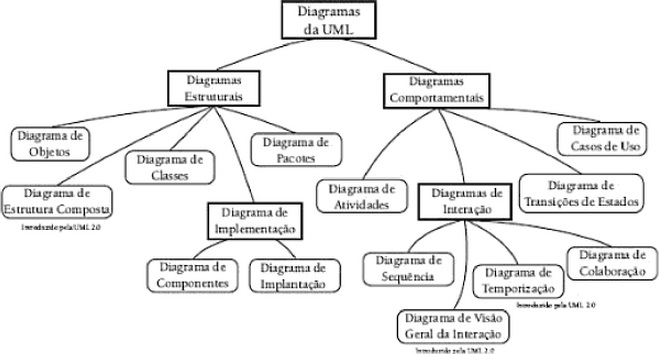
\includegraphics[scale=0.8]{./imagens/1_q_teorico/qt4.png}}
				\caption[Principais Diagramas definidos pela UML.]{Diagramas definidos pela
				UML. \textbf{Fonte:}\citeonline{2015principios}}
				\label{fig:qt4}
		\end{figure}
		
		\pagebreak
		\par A linguagem de modelagem UML não é um processo rígido e permite uma
		adequação de acordo com a situação do projeto em que é aplicada. Por permitir
		essa flexibilidade e prover suporte adequado para determinados casos de um
		projeto, será utilizada a linguagem de modelagem UML  para o desenvolvimento
		desta pesquisa.
\subsection{Processos de \textit{Software}}
	
	
	\par Segundo \citeonline[p.52]{pressman2011}, um processo de \textit{software} é
“uma metodologia para as atividades, ações e tarefas necessárias para
desenvolver um \textit{software} de alta qualidade”.

	\par Para \citeonline{sommerville2003}, não existe um processo ideal, pois isso
dependerá de cada projeto, possibilitando cada qual implementar algum modelo já
existente. Contudo \citeonline{pressman2011} afirma que uma metodologia
genérica possui cinco passos:
	\begin{itemize}
	  
	  \item Comunicação: antes de iniciar os trabalhos técnicos deve-se entender
	  os objetivos do sistema e levantar requisitos para o bom funcionamento do
	  \textit{software}.
	  
	  \item Planejamento: cria um plano de projeto, que conterá as tarefas a
	  serem seguidas, riscos prováveis e recursos necessários.
	  
	  \item Modelagem: esboça o sistema para que se tenha uma ideia de como ele
	  deverá ficar e como encontrar a melhor solução para desenvolvê-lo.
	  
	  \item Construção: é a etapa de desenvolvimento e testes.
	  
	  \item Emprego: o \textit{software} pronto em sua totalidade ou parcialmente
	  é implantado no cliente e este retorna o seu \textit{feedback}.
	 
	 \end{itemize}
	 
	 \par Dessa forma, normalmente qualquer um dos modelos (ciclo de vida clássico,
evolutivo ou espiral) utilizaram os princípios das metodologias acima citadas.
%GCM
%\section{\textbf{Google Cloud 	Messaging}}

	\par Para que os alunos sejam notificados quando houver alguma mudança no
portal do aluno, será utilizada uma API oferecida pela Google denominada
\textit{Google Cloud Messaging} ou simplesmente GCM, um recurso que tem por
objetivo notificar as aplicações \textit{Android}. Segundo \citeonline{leal2014}, ele
permite que aplicações servidoras possam enviar pequenas mensagens de até 4
KB\footnote{\textit{KB - Kilobytes}} para os aplicativos móveis, sem que este
necessite estar em execução. Ainda de acordo com \citeonline{leal2014} para o
bom funcionamento do recurso apresentado, são necessários os seguintes
componentes:

\begin{itemize}
	
	\item \textit{Sender ID\footnote{Identity}}: é o identificador do projeto.
	Será utilizado pelo servidores da Google para identificar a aplicação
	que envia a mensagem.
	
	\item \textit{Application ID}: é o identificador da aplicação \textit{Android}. O
	identificador é o nome do pacote do projeto que consta no
	\texttt{AndroidManifest.xml}.
	
	\item \textit{Registration ID}: é o identificador gerado pelo servidor GCM
	quando aplicação \textit{Android} se conecta a ele. Este deve ser enviado
	também à aplicação servidora.
	
	\item \textit{Sender Auth Token}: é uma chave que é incluída no cabeçalho
	quando a mensagem é enviada da aplicação servidora para o GCM. Essa chave serve
	para que a API da Google possa enviar as mensagens para o dispositivo
	correto.

\end{itemize}

	\par De acordo com os componentes acima citados, quando uma aplicação servidora
enviar uma mensagem para o aplicativo \textit{Android}, na verdade está
enviando para o servidor GCM que será encarregado de enviar a mensagem para a aplicação
\textit{mobile}.

%jersey
%\section{\textit{Jersey}}

	\par Atualmente um padrão para desenvolvimento de serviços \textit{web} vem
sendo bastante adotado, trata-se do padrão arquitetural REST. De acordo com
\citeonline{saudate2012}, a linguagem \textit{Java} possui uma especificação
própria para desenvolvimento de serviços REST desde de setembro de 2008, que é
a JSR311, ou como é popularmente chamado JAX-RS. Esta especificação provê um
conjunto de API's simples, para facilitar o desenvolvimento de serviços
\textit{web}. De acordo com \citeonline{oracle22015} "JAX-RS é uma API da
linguagem de programação \textit{Java} projetada para tornar mais fácil
desenvolver aplicações que usam a arquitetura REST"\footnote{Tradução e resumo
de informações de responsabilidade dos autores da pesquisa.}. Através desta
especificação torna-se mais facíl e ágil a contrução de serviços \textit{web}
baseados em REST.

	\par Como JAX-RS é apenas uma especificação, ela necessita então de uma
implementação. Uma das implementações desta especificação é o
\textit{framework Jersey}. Segundo \citeonline{oracle2015} "\textit{Jersey}, a
implementação de referência de JAX-RS, implementa suporte para as anotações
definidas no JSR 311, tornando mais fácil para os desenvolvedores a construir
serviços \textit{Web RESTful} usando a linguagem de programação
\textit{Java}"\footnote{Tradução e resumo de informações de responsabilidade
dos autores da pesquisa.}. Além das anotações que facilitam seu uso,
\textit{Jersey} pode prover serviços com uma infinidade de tipos de
mídias, tais como XML e JSON entre outros.

	\par O \textit{framework Jersey} tem amplo suporte para os varios métodos HTTP.
Fazendo uso dele pode-se facilmente implementar recursos REST. Além disso o
\textit{Jersey}  pode rodar tanto em servidores que implementem a especificação
\textit{Servlet} ou não. Este \textit{framework} será usado para contruir a
parte responsável por prover os serviços para o aplicativo \textit{Android}.
%hibernate
%\section{Hibernate}

	\par Com a evolução e popularização da linguagem Java, e com o seu
uso cada vez maior em ambientes corporativos, percebeu-se que se perdia muito
tempo com a confecção de \textit{queries} SQL usadas nas consultas em bancos de
dados relacionais e com a construção do código JDBC\footnote{JDBC -
\textit{Java Database Connectivity}}, que era responsável por trabalhar com
estas consultas. Além disso era notório que, mesmo a linguagem SQL sendo
padronizada, ela apresentava diferenças significativas entre os diversos bancos
de dados existentes. Isso fazia com que a implementação de um software ficasse
amarrada em um banco de dados específico e era extremamente custosa uma mudança
poterior. Além disso havia o problema de lidar diretamente com dois paradigmas
um pouco diferentes: o orientado a objeto e o relacional. Com o intuito de
resolver estes problemas, é que surgiram os \textit{frameworks}
ORM\footnote{ORM - \textit{Object-relational Mapping}} tais como Hibernate,
EclipseLink, Apache OpenJPA entre outros.

	\par Conforme surgiam novas alternativas e implementações para sanar esses
problemas, surgia um novo problema: a falta de padronização entre os
\textit{frameworks} de ORM. Para resolver esse problema foi criada o
JPA\footnote{JPA - \textit{Java Persistence API}} que, de acordo com
\citeonline[p.12]{keith2009pro}, "nasceu do reconhecimento das demandas dos
profissionais e as existentes soluções proprietárias que eles estavam usando
para resolver os seus problemas"\footnote{Tradução de responsabilidade dos
autores da pesquisa.}. 
	
	\par A especificação JPA foi concebida sendo a terceira parte da
especificação EJB\footnote{EJB - \textit{Enterprise Java Bean}}, e deveria
atender ao propósitos de persistêcia de dados desta especificação.
De acordo com \citeonline[p.12]{keith2009pro}, JPA é um \textit{framework} leve
baseado em POJO's\footnote{POJO - \textit{Plain Old Java Object }}, para
persistência de dados em Java e que, embora o mapeamento objeto
relacional seja seu principal componente, ele ainda oferece soluções de
arquitetura para aplicações corporativas escaláveis\footnote{Tradução e resumo
de informações de responsabilidade dos autores da pesquisa.}.

	\par O \textit{framework} Hibernate é uma das implementações da especificação
JPA. De acordo com \citeonline{sourceforgeHibernate2015}, o Hibernate é
uma ferramenta de mapeamento relacional, muito popular entre aplicações
Java e implementa a \textit{Java Persistence API}. Foi criado por uma
comunidade de desenvolvedores, do mundo todo, que eram liderados por Gavin King.
De acordo com \citeonline{hibernate2015} "o Hibernate cuida do mapeamento
de classes Java para tabelas de banco de dados, e de tipos de dados
Java para tipos de dados SQL".

	\par O Hibernate está bastante difundido na comunidade de desenvolvedores Java
ao redor do mundo, pelo fato de ser simples de usar e por evitar esforços
desnecessários na parte de infraestrutura das aplicações onde é usado, mantendo
assim o foco na lógica de negócio. As pricipais vantagens do uso do Hibernate,
segundo \citeonline{sourceforgeHibernate2015}, são:

	\begin{itemize}
	  
		\item Provedor JPA: além de sua API nativa , o Hibernate também é uma
		implentação da especificação JPA, podendo assim ser facilmente usado em
		qualquer ambiente JPA.
		  		
		\item Persistência idiomática: permite que sejam construídas classes
		persistentes, e que suportem herança e polimorfismo entre outras estratégias,
		sem a necessidade da contrução de estruturas especiais para tal fim.
			  	
		\item \textit{Performance} e suporte: permite que sejam usadas várias
		estratégias de inicialização. Além disso não necessita de tabelas especiais
		no banco de dados. Mostra-se vantajoso também por gerar a maior parte do SQL
		necessário e evitar esforço desnecessário por parte do desenvolvedor, além de
		ser mais rápido que o JDBC puro.
		  
		\item Escalável: o Hibernate foi projetado para trabalhar em
		\textit{clusters} de servidores de aplicações e oferecer uma estrutura muito
		escalável, que se comporta bem tanto com número pequeno de usuários até
		números mais elevados.
	
		\item Confiável: sua confiabilidade e estabilidade são comprovadas pelo seu
		grande uso e aceitação atualmente.
				
		\item Extensível: Hibernate é altamente configurável e
		extensível\footnote{Tradução e resumo de informações de responsabilidade dos
		autores da pesquisa.}.
	
	\end{itemize}
	
	\par O Hibernate será usado nesta pesquisa com o intuito de fazer a
gerência dos dados coletados e que serão providos para o aplicativo
Android através do \textit{web service}, em conjunto com o banco de
dados.
\chapter{QUADRO METODOLÓGICO}

	\par Neste capítulo serão apresentados os métodos adotados para se realizar
	esta pesquisa, tais como tipo de pesquisa, contexto, procedimentos, entre outros.
	
	%tipo de pesquisa
	\section{Tipo de pesquisa}
		\section{Tipo de pesquisa}
	
	\par Uma pesquisa é o ato de buscar e procurar pela resposta de algo.
\citeonline[p. 15]{markoni2002} definem pesquisa como “uma indagação minuciosa
ou exame crítico e exaustivo na procura de fatos e princípios”.

	\par Existem diversos tipos de pesquisa, no entanto percebeu-se que para o
propósito desta, a mais indicada foi a pesquisa aplicada, pois está se
desenvolvendo um projeto real que poderá ser utilizado por qualquer instituição
de ensino, mas que não mudará a forma com que as pessoas recebam suas
informações, apenas acrescentará mais uma opção de consultá-las.

	\par Segundo \citeonline[p. 15]{markoni2002}, uma pesquisa do tipo aplicada
“caracteriza-se por seu interesse prático, isto é, que os resultados sejam
aplicados ou utilizados, imediatamente, na solução de problemas que ocorrem na
realidade”.

	\par Dessa maneira, percebeu-se que esta pesquisa enquadra-se no tipo de pesquisa
aplicada, pois com a execução da mesma resolve um problema específico, e para
isso está desenvolvendo-se um aplicativo para dispositivos móveis que facilitará aos
graduandos acessarem o sistema \textit{web} de uma universidade.
	
	%contexto de pesquisa
	\section{Contexto de pesquisa}
		%\section{Contexto de pesquisa}

	\par Para que os alunos possam saber suas notas, faltas e provas agendadas,
é necessário que eles acessem o portal do aluno para consultá-las.

	\par O \textit{web service}, criado através desta pesquisa, tem por objetivo
fornecer a estrutura para que a Univás possa disponibilizar suas informações
através de serviços, bem como desenvolver um serviço para que o aplicativo
consulte as notas, faltas e provas agendadas dos alunos.

	\par A aplicação Android, por sua vez, tem por finalidade facilitar aos
estudantes o acesso às suas informações escolares mais procuradas.
	
	\par Os alunos acessarão o aplicativo com o mesmo usuário e senha do
portal do aluno, e quando houver o lançamento de alguma nota ou prova agendada,
eles serão notificados em seu dispositivo. Ao clicar na notificação
o sistema apresentará a informação recebida. 
	
	%instrumentos
	\section{Instrumentos}
		%\section{Instrumentos}

	\par Os instrumentos de pesquisa existem para que se possam levantar
informações para realizar um determinado projeto.

	\par Pode-se dizer que um questionário é uma forma de coletar
informações através de algumas perguntas feitas a um público específico.
Segundo \citeonline{gunther2003}, o questionário pode ser definido como
um conjunto de perguntas que mede a opinião e interesse do respondente.

	\par Neste trabalho foi realizado um questionário simples, apresentado na
Figura \ref{fig:qm1}, contendo quatro perguntas e enviado para \textit{e-mails}
de alguns alunos da universidade. O foco desse questionário era saber o motivo
pelo qual os usuários mais acessavam o portal do aluno e se tinham alguma
dificuldade em encontrar o que procuravam. Obteve-se um total de treze
respostas, no qual pode-se perceber que a maioria dos entrevistados afirmaram
ter dificuldades para encontrar as informações de que necessitam, e que
gostariam de ser notificados quando houvesse alguma atualização de notas. Sobre
o motivo do acesso, cem por cento dos discentes responderam que entram no
sistema \textit{web} para consultar os resultados das avaliações.

\begin{figure}[h!]
	\centerline{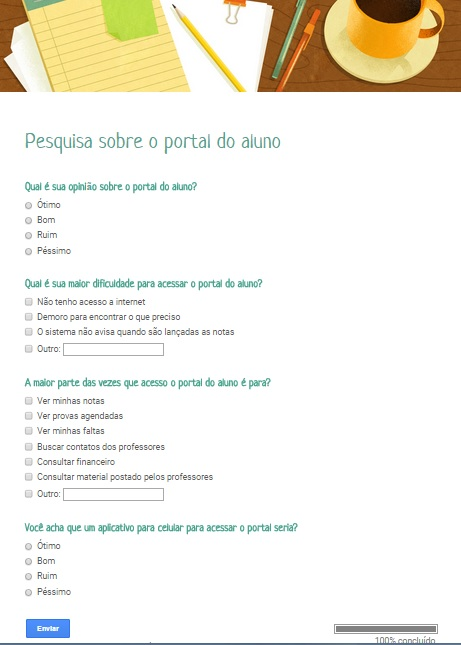
\includegraphics[scale=0.5]{./imagens/2_q_metodologico/qm1.png}}
	\caption[Quetionário Aplicado]{Quetionário Aplicado.
		\textbf{Fonte:}Elaborado pelos autores.}
	\label{fig:qm1}
\end{figure}
	

	\par Outro instrumento utilizado para realizar esta pesquisa foram as reuniões,
ou seja, reunir-se com uma ou mais pessoas em um local, físico ou remotamente
para tratar algum assunto específico. Para \citeonline{ferreira1999}, reunião é o ato de
encontro entre algumas pessoas em um determinado local, com finalidade de tratar
qualquer assunto.

	\par Durante a pesquisa, foram realizadas reuniões entre os participantes com
o objetivo de discutir o andamento das tarefas pela qual cada integrante responsabilizou-se
a fazer e traçar novas metas. Também foram utilizadas referências
de livros, revistas, manuais e \textit{web sites}.
	
	%Procedimentos e resultados
	\section{Procedimentos e Resultados}
		%\section{Procedimentos e Resultados}

	
			%Modelagem
			\subsection{Modelagem}
				%\subsection{Modelagem}
	
	\par Para atender o objetivo proposto por esta pesquisa, necessitou-se antes
modelar o \textit{software} através dos diagramas de UML.

	
			%gcm
			\subsection{Google Cloud Messaging}
				%\subsection{\textit{Google Cloud Messaging}}

	\par O envio dos dados do \textit{web service} para o aplicativo
\textit{Android}, é feito através de um serviço da \textit{Google} conhecido
como GCM.

	\par Para que o serviço apresente o resultado esperado, foi preciso acessar o
\textit{site} da \textit{Google Developers Console} e criar um novo projeto. Ao
criá-lo, foi necessário ir na aba API's e ativar a opção \textit{Google Cloud
Messaging for Android}.

 	\par Com a criação do projeto, a \textit{Google} oferece um número que
identificará o \textit{software}, também chamado de \texttt{Sender ID},
conforme mostra a Figura \ref{fig:gcm}.


	\begin{figure}[h!] 
		\centerline{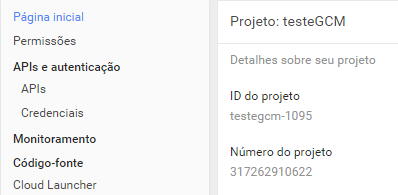
\includegraphics[scale=1]{./imagens/2_q_metodologico/4_procedimentos_resultados/41_gcm/gcm.png}}
		\caption[\texttt{Sender ID} do GCM]{\texttt{Sender ID} do GCM.
		\textbf{Fonte:}Elaborado pelos autores.}
		\label{fig:gcm}
	\end{figure}
	\pagebreak
	
	\par Por fim, acessou-se a aba Credenciais para indicar o IP do servidor. Ao
informa-lo, o serviço gerou uma chave pública a qual foi inserida no
\textit{web service}. Na Figura \ref{fig:gcm1}, é possível ver o código de
acesso criado.


	\begin{figure}[h!] 
		\centerline{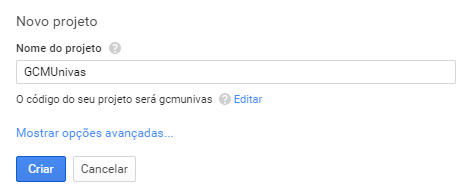
\includegraphics[scale=0.5]{./imagens/2_q_metodologico/4_procedimentos_resultados/41_gcm/gcm1.png}}
		\caption[Geração da credencial do GCM]{Geração da credencial do GCM.
		\textbf{Fonte:}Elaborado pelos autores.}
		\label{fig:gcm1}
	\end{figure}
	
			%Aplicativo
			\subsection{Aplicativo}
				%\subsection{Aplicativo}

	\par O primeiro passo realizado para a construção do aplicativo Android, foi a
modelagem do software através dos diagramas de UML, que permitiram nortear o
desenvolvimento.

	\par A princípio projetou-se um diagrama para se ter uma visão geral do
aplicativo. Nele pode-se ver a arquitetura da aplicação, bem como a comunicação
com o GCM e o \textit{web service}.

	\par Quando o servidor precisa enviar uma informação para os dispositivos
móveis, ele envia a mensagem ao GCM, que a transfere para aplicativo. Ao
receber os dados, a classe \texttt{GcmBroadcastReceiverUnivas} executa a classe
\texttt{GcmIntentServiceUnivas} que por sua vez irá notificar o usuário,
contudo antes de notificá-lo, ela envia as informações para a classe
\texttt{HttpUtil}, que faz a conversão dos dados vindos em JSON para o formato
da classe \texttt{EventTO}. Ao finalizar a leitura e conversão dos elementos,
as informações são enviadas para a classe \texttt{DatabaseExecute} que realiza
a gravação dos dados no banco de dados.

	\par Quando o usuário clica na notificação, é apresentada a ele uma
\textit{activity} a qual exibe as informações recebidas. Neste contexto, quando
o evento recebido se tratar de uma nota será aberta a \textit{activity}
\texttt{NotificationResultsActivity}, no caso de ser uma falta é executada a
\textit{activity} \texttt{NotificationFoulsActivity} e caso for um evento de
provas agendadas então é mostrada a \textit{activity}
\texttt{NotificationAgendasActivity}.

	\par Para o estudante visualizar suas informações, ele acessará a classe
\texttt{MainActivity}. Se desejar ver as suas notas, então é apresentada a
\textit{activity} \texttt{ListResultsActivity}, que utiliza a classe
\texttt{ListResultsAdapter} para gerenciar as informações e apresentá-las ao
discente. No entanto, se escolher a opção de faltas, é apresentada a
\textit{activity} \texttt{ListFoulsActivity}, que receberá as informações da
classe \texttt{ListFoulsAdapter} e caso decida-se pela opção provas agendadas é
exibida a \textit{activity} \texttt{ListAgendasActivity}, gerenciada pela
classe \texttt{ListAgendasAdapter}.

	\par A classe \texttt{GcmControllerUnivas}, tem por finalidade cadastrar o
dispositivo no GCM e enviar a chave gerada para o \textit{web service}. Na
Figura \ref{fig:app}, é apresentado o diagrama de arquitetura.

	\begin{figure}[h!] 
		\centerline{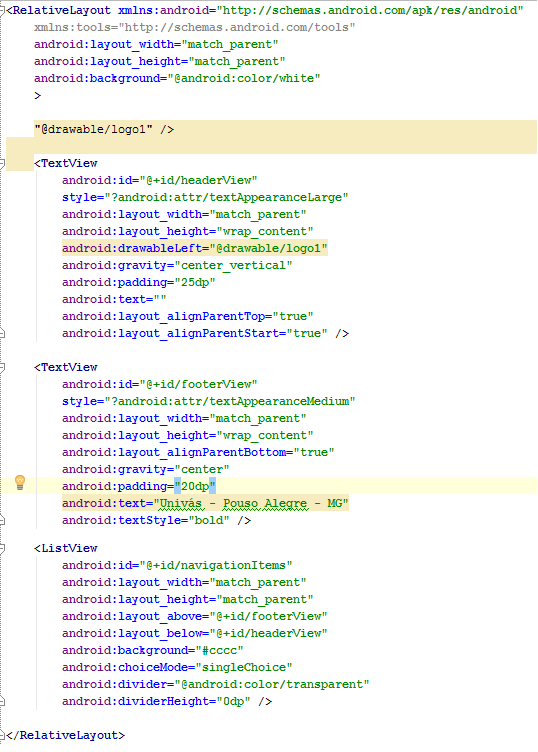
\includegraphics[scale=0.42]{./imagens/2_q_metodologico/4_procedimentos_resultados/42_aplicativo/app.png}}
		\caption[Diagrama de arquitetura do aplicativo]{Diagrama de arquitetura do aplicativo.
		\textbf{Fonte:}Elaborado pelos autores.}
		\label{fig:app}
	\end{figure}
	
	\par Posteriormente, foi desenvolvido o diagrama de caso de usos, com
finalidade em ter uma visão das funcionalidades do software pelo lado do
usuário. O utilitário permite ao aluno receber notificações quando for lançada
uma nova nota, falta ou prova agendada e visualizar estas informações. Na
Figura \ref{fig:app1} é possível ver o diagrama de casos de uso.

	\begin{figure}[h!] 
		\centerline{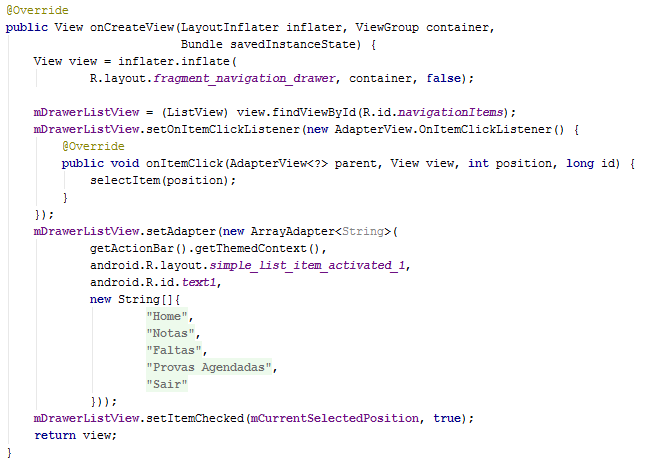
\includegraphics[scale=0.7]{./imagens/2_q_metodologico/4_procedimentos_resultados/42_aplicativo/app1.png}}
		\caption[Diagrama de casos de uso]{Diagrama de casos de uso.
		\textbf{Fonte:}Elaborado pelos autores.}
		\label{fig:app1}
	\end{figure}
	
	\par Para iniciar a construção do aplicativo, fez-se necessário a instalação e
configuração do ambiente de desenvolvimento. Primeiramente, realizou-se o
\textit{download} da IDE Android Studio, versão 1.1.0 e do Android SDK, versão
24.0.2, ambos no site \textit{Developers} Android através do endereço
\url{https://developer.android.com/intl/pt-br/sdk/index.html}.

	\par Contudo, ao executar o emulador do Android o sistema apresentava a
seguinte mensagem: “\textit{emulator: Failed to open the HAX device!}”. Depois
de algum tempo pesquisando, percebeu-se que era necessário instalar um programa
chamado Intel \textit{Hardware Accelerated Execution Manager} (HAXM), que
permite a execução do emulador Android mais rápido.

	\par No entanto, ao instalá-lo ocorria o seguinte erro: “\textit{this computer
meets the requirements for haxm but intel virtualization technology (VT-x) is
not turned on.}” A solução foi acessar a BIOS da máquina e habilitar o
assistente de hardware para virtualização. Daí em diante, foi possível executar
no emulador as aplicações feitas no Android Studio.

	\par Com o ambiente já configurado, houve a necessidade de se criar um
repositório no controlador de versão Github, o qual pode ser acessado através
do endereço \url{https://github.com/diegodnunes12/AppTCC} e compartilhado entre
os participantes do projeto.

	\par A partir de então, passou-se a desenvolver o software. A princípio, foi
construída uma \textit{activity}, que é acessível ao aluno logo que a aplicação
se inicia. Essa \textit{activity} é do tipo \textit{Navigation Drawer Layout},
ou seja, é um painel que permite inserir as opções de navegação do aplicativo,
semelhante a um menu.	Ao criar essa \textit{activity}, o Android Studio gera
automaticamente a classe \texttt{NavigationDrawerFragment} e um arquivo XML na
pasta \textit{layout}, chamado \texttt{fragment\_navigation\_drawer.xml}.

	\par No arquivo \texttt{fragment\_navigation\_drawer.xml} foram inseridos três
\textit{widgets}, sendo dois do tipo \texttt{textView}, para o cabeçalho com a
logomarca da Univás e para o rodapé com o seguinte texto: “Univás – Pouso
Alegre – MG” e um \textit{widget} do tipo \texttt{listView} que contém a lista
com as opções que o software oferece ao aluno.

	\par O \textit{layout} desta \textit{activity} chama-se
\textit{relativeLayout}, o qual permite um elemento ser posicionado em relação
a um outro. Desta forma o \textit{widget} \textit{listView} do Android, utiliza
a propriedade \texttt{android:layout\_below="@+id/headerView"} para se posicionar abaixo do
componente com id \textit{headerView} e a propriedade
\texttt{android:layout\_above="@+id/footerView"} indicando que ela deve preceder
o \textit{widget} com id \textit{footerView}. Na Figura \ref{fig:app2}, pode
ser visto o código XML dos \textit{widgets} desta tela.

	\begin{figure}[h!] 
		\begin{lstlisting}[style=custom_XML]
	<RelativeLayout xmlns:android="http://schemas.android.com/apk/res/android"
    xmlns:tools="http://schemas.android.com/tools"
    android:layout_width="match_parent"
    android:layout_height="match_parent"
    android:background="@android:color/white">
	    <TextView
	        android:id="@+id/headerView"
	        style="?android:attr/textAppearanceLarge"
	        android:layout_width="match_parent"
	        android:layout_height="wrap_content"
	        android:drawableLeft="@drawable/logo1"
	        android:gravity="center_vertical"
	        android:paddingTop="5dp"
	        android:paddingBottom="5dp"
	        android:paddingLeft="25dp"
	        android:paddingRight="25dp"
	        android:text=""
	        android:layout_alignParentTop="true"
	        android:layout_alignParentStart="true" />
	    <TextView
	        android:id="@+id/footerView"
	        style="?android:attr/textAppearanceMedium"
	        android:layout_width="match_parent"
	        android:layout_height="wrap_content"
	        android:layout_alignParentBottom="true"
	        android:gravity="center"
	        android:padding="20dp"
	        android:textColor="#228B22"
	        android:text="Univas - Pouso Alegre - MG"
	        android:textStyle="bold" />
	    <ListView
	        android:id="@+id/navigationItems"
	        android:layout_width="match_parent"
	        android:layout_height="match_parent"
	        android:layout_above="@+id/footerView"
	        android:layout_below="@+id/headerView"
	        android:background="#228B22"
	        android:choiceMode="singleChoice"
	        android:divider="@android:color/transparent"
	        android:dividerHeight="1dp" />
</RelativeLayout>
\end{lstlisting}
		\caption[Código dos widgets do arquivo
		fragment\_navigation\_drawer.xml]{Código dos \textit{widgets} do arquivo
		\texttt{fragment\_navigation\_drawer.xml}.
		\textbf{Fonte:}Elaborado pelos autores.}
		\label{fig:app2}
	\end{figure}
	
	\pagebreak
	
	\par A classe \texttt{NavigationDrawerFragment} representa o painel de
navegação. Nela se destaca o método \texttt{onCreateView()}, responsável por
criar o \textit{layout} de navegação. Na Figura \ref{fig:app3}, é mostrado o
método \texttt{onCreateView()} informando ao sistema operacional o \textit{layout} a
ser carregado e adicionando a um \textit{array} de \textit{String} as
alternativas de navegação que serão exibidos no \textit{listView} da tela
principal. Pode-se perceber também o método \texttt{onItemClick()}, que é
executado no momento em que o usuário clica em algum item da lista. 
	


	\begin{figure}[h!] 
		\begin{lstlisting}[style=custom_JAVA]
@Override
public View onCreateView(
		LayoutInflater inflater, ViewGroup container,Bundle savedInstanceState) {
    View view = inflater.inflate(
            R.layout.fragment_navigation_drawer, container, false);

    mDrawerListView = (ListView) view.findViewById(R.id.navigationItems);
    mDrawerListView.setOnItemClickListener(new AdapterView.OnItemClickListener() {
        @Override
        public void onItemClick(AdapterView<?> parent, View view, int position, long id) {
            selectItem(position);
        }
    });
    mDrawerListView.setAdapter(new ArrayAdapter<String>(
            getActionBar().getThemedContext(),
            android.R.layout.simple_list_item_activated_1,
            android.R.id.text1,
            new String[]{
                    getString(R.string.title_section1),
                    getString(R.string.title_section2),
                    getString(R.string.title_section3),
                    getString(R.string.title_section4),
                    getString(R.string.title_section5)
            }));
    mDrawerListView.setItemChecked(mCurrentSelectedPosition, true);
    return view;
}
public boolean isDrawerOpen() {
    return mDrawerLayout != null && mDrawerLayout.isDrawerOpen(mFragmentContainerView);
}
\end{lstlisting}
		\caption[Método onCreateView()]{Método \texttt{onCreateView()}.
		\textbf{Fonte:}Elaborado pelos autores.}
		\label{fig:app3}
	\end{figure}
	
	\pagebreak
	
	\par Nesse caso, quando for selecionada alguma opção da tela principal será
executado o método \texttt{selectItem()} apresentado na Figura \ref{fig:app4}, o
qual é responsável por retornar a posição do \textit{array} em que se encontra a
opção selecionada pelo aluno.
	
	\begin{figure}[h!] 
		\begin{lstlisting}[style=custom_JAVA]
	private void selectItem(int position) {
        mCurrentSelectedPosition = position;
        if (mDrawerListView != null) {
            mDrawerListView.setItemChecked(position, true);
        }
        if (mDrawerLayout != null) {
            mDrawerLayout.closeDrawer(mFragmentContainerView);
        }
        if (mCallbacks != null) {
            mCallbacks.onNavigationDrawerItemSelected(position);
        }
    }
\end{lstlisting}
		\caption[método selectItem()]{método \texttt{selectItem()}.
		\textbf{Fonte:}Elaborado pelos autores.}
		\label{fig:app4}
	\end{figure}
	
	\par O próximo passo foi criar o banco de dados do aplicativo para salvar as
informações recebidas do \textit{web service}. Para que isso fosse possível,
elaborou-se uma classe denominada \texttt{DatabaseHelper} que estende da classe
\texttt{SQLiteOpenHelper} do Android, com dois métodos, um chamado
\textit{onCreate()} que cria a estrutura do banco de dados e outro conhecido
por \textit{onUpgrade()}, usado se for necessário atualizar a estrutura do
banco de dados.

	\par Foi preciso criar um atributo que mantém a versão do banco de dados. Essa
informação serve para que o Android consiga saber qual dos dois métodos devem
ser executados. Ao iniciar a aplicação pela primeira vez, estando a versão em 1
(um), o sistema chamará o método \texttt{onCreate()}. Se for preciso atualizar
a estrutura do banco, o atributo versão deve ser incrementado em 1 (um), de
modo que ao executar o software o sistema operacional perceba a mudança,
chamando o método \texttt{onUpgrade()}. Na Figura \ref{fig:app5} é apresentado a
classe \texttt{DatabaseHelper}.

	\begin{figure}[h!] 
		\begin{lstlisting}[style=custom_JAVA]
public class DatabaseHelper extends SQLiteOpenHelper {

    private static final String BANCO_DADOS = "univasDB";
    private static int VERSAO = 1;

    public DatabaseHelper(Context context) {
        super(context, BANCO_DADOS, null, VERSAO);
    }
    @Override
    public void onCreate(SQLiteDatabase db) {
        db.execSQL("CREATE TABLE disciplinas (_id LONG PRIMARY KEY, nome TEXT);");

        db.execSQL("CREATE TABLE eventos (_id LONG PRIMARY KEY, id_disciplina LONG, " +
                " tipo_evento TEXT, descricao_evento TEXT," +
                " data_evento TEXT, valor_evento INTEGER, nota INTEGER,"  +
                " FOREIGN KEY (id_disciplina) REFERENCES disciplinas (_id) );");
    }
    @Override
    public void onUpgrade(SQLiteDatabase db, int i, int i2) {
        //Nao ha atuaizacoes no momento
    }
}
\end{lstlisting}
		\caption[Classe DatabaseHelper]{Classe \texttt{DatabaseHelper}.
		\textbf{Fonte:}Elaborado pelos autores.}
		\label{fig:app5}
	\end{figure}
	
	\par Em seguida foi criada a classe responsável por executar as consultas SQL,
denominada \texttt{DatabaseExecute}. Nela foram inseridos os métodos
responsáveis por inserir, alterar e buscar os dados dos alunos no banco de
dados local do aplicativo. Na Figura \ref{fig:app6}, pode-se observar o método
que possibilita a inserção dos eventos ocorridos. Esses eventos podem ser
notas, faltas ou provas agendadas.
	
	
	\begin{figure}[h!] 
		\begin{lstlisting}[style=custom_JAVA]
public void insertEvents(EventTO to){
        SQLiteDatabase db = helper.getWritableDatabase();

        ContentValues values = new ContentValues();
        values.put("_id", to.get_id());
        values.put("id_disciplina", to.getId_discipline());
        values.put("tipo_evento", to.getType_event());
        values.put("descricao_evento", to.getDescription_event());
        values.put("data_evento", to.getDate_event());
        values.put("valor_evento", to.getValue_event());
        values.put("nota", to.getResult());

        long result = db.insert("eventos", null, values);

        if(result != -1 ){
            Log.d(TAG, " Evento salvo com sucesso!");
        }else{
            Log.d(TAG, " Erro ao salvar o Evento!");
        }
    }
\end{lstlisting}
		\caption[Método de inserção de eventos]{Método de inserção de eventos.
		\textbf{Fonte:}Elaborado pelos autores.}
		\label{fig:app6}
	\end{figure}
	
	\pagebreak
	
	\par Este método recebe um objeto da classe \texttt{EventTO} com os elementos
necessários para inserir o evento no banco de dados. Para que seja possível a
inserção dos dados, \citeonline{monteiro2012}, afirma que é necessário
recuperar a referência da classe \texttt{SQLiteDatabase} através do método
\texttt{getWritableDatabase()}, logo após é instanciada a classe
\texttt{ContentValues}, onde são informados os campos da tabela e os
respectivos valores. Ao concluir, é chamado o \texttt{insert()} da classe
\texttt{SQLiteDatabase} informando o nome da tabela e o objeto da classe
\texttt{ContentValues}.

	\par Para listar os resultados dos exames realizados pelos discentes no painel
de notas é utilizado o método \texttt{getResults()} que retorna uma lista de
objetos da classe \texttt{EventTO}. De acordo com \citeonline{monteiro2012},
para conseguir recuperar as informações armazenadas no banco de dados é preciso
adquirir a instância de leitura da classe \texttt{SQLiteDatabase} através do
método \texttt{getReadableDatabase()}. Por meio dele pode-se realizar a
consulta, que devolve um \textit{Cursor} para navegar pelos resultados. Por
fim, é composto um objeto do tipo \texttt{EventTO} e inserido na lista. Na
Figura \ref{fig:app7} é apresentado o método \texttt{getResults()}.

	\par Foram inseridos mais dois métodos semelhantes ao \texttt{getResults()},
que são os métodos de \texttt{getFouls()} e \texttt{getAgendas()} para
recuperar as faltas e provas agendadas respectivamente. O que diferencia-os é a
consulta SQL, já que no \texttt{getFouls()}  foram buscados os dados onde o
\texttt{tipo\_evento = ‘FALTAS'} e no \texttt{getAgendas()} onde o
\texttt{tipo\_evento = ‘PROVA\_AGENDADA'}.

	\begin{figure}[h!] 
		\begin{lstlisting}[style=custom_JAVA]
public List<EventTO> getResults(){
        List<EventTO> notasTO = new ArrayList<>();

        SQLiteDatabase db = helper.getReadableDatabase();
        Cursor cursor =
                db.rawQuery("SELECT _id, id_disciplina, descricao_evento, valor_evento, nota  FROM" +
                                " eventos WHERE tipo_evento = 'PROVA_APLICADA'",
                        null);
        cursor.moveToFirst();

        for(int i = 0; i<cursor.getCount();i++){
            EventTO nota = new EventTO();

            nota.set_id(cursor.getLong(0));
            nota.setId_discipline(cursor.getLong(1));
            nota.setDescription_event(cursor.getString(2));
            nota.setValue_event(cursor.getInt(3));
            nota.setResult(cursor.getInt(4));

            notasTO.add(nota);
            cursor.moveToNext();
        }
        cursor.close();
        return notasTO;
    }
\end{lstlisting}
		\caption[Método getResults()]{Método \texttt{getResults()}.
		\textbf{Fonte:}Elaborado pelos autores.}
		\label{fig:app7}
	\end{figure}
	
	\pagebreak
	
	\par A fim de estabelecer uma conexão entre o aplicativo e o \textit{web
service}, foi preciso conceder a permissão de acesso à internet no arquivo
\texttt{AndroidManifest.xml} da seguinte forma: \texttt{<uses-permission
android:name="android.permission.INTERNET" />}.

	\par Logo após, criou-se uma classe chamada de \texttt{HttpUtilUnivas} para ler
informações recebidas do \textit{web service}. Ela estende da classe
\texttt{AsyncTask} que executa a consulta em paralelo com a \textit{thread
main}, evitando travar a aplicação enquanto recebe as informações vindas do
\textit{web service}. Estes dados estão em formato JSON e foi utilizada a
biblioteca GSON para convertê-las para o formato da classe \texttt{EventTO}.
Após a leitura, o objeto da classe \texttt{EventTO} é enviado para a classe
\texttt{DatabaseExecute}, a fim de realizar a inserção os dados no banco. A
Figura \ref{fig:app8}, mostra a classe \texttt{HttpUtilUnivas}.

	\begin{figure}[h!] 
		\begin{lstlisting}[style=custom_JAVA]
try{
        HttpClient httpClient = new DefaultHttpClient();
        HttpGet request = new HttpGet();
        request.setURI(new URI(urlEvents));

        HttpResponse response = null;
        try {
            response = httpClient.execute(request);
        } catch (IOException e) {
            e.printStackTrace();
        }
        InputStream content = null;
        try {
            content = response.getEntity().getContent();
        } catch (IOException e) {
            e.printStackTrace();
        }
        Reader reader = new InputStreamReader(content);
        Gson gson = new Gson();
        returnEvents = gson.fromJson(reader, Events.class);

        for (int i = 0; i< returnEvents.getEventos().size(); i++){
            DatabaseExecute execute = new DatabaseExecute(helper);
            EventTO to = new EventTO();
            to.set_id((long) returnEvents.getEventos().get(i).getId_evento());
            to.setValue_event(returnEvents.getEventos().get(i).getValor());
            to.setDescription_event(returnEvents.getEventos().get(i).getDescricao());
            to.setId_discipline(returnEvents.getEventos().get(i).getId_disciplina());
            to.setDate_event(returnEvents.getEventos().get(i).getData());
            to.setResult(returnEvents.getEventos().get(i).getNota());
            to.setType_event(returnEvents.getEventos().get(i).getTipoEvento());

            if(execute.existingEvent(to.get_id()) == false){
                execute.insertEvents(to);
            }else{
                execute.updateEvent(to);
            }
        }
        content.close();
    } catch (URISyntaxException e) {
        e.printStackTrace();
    } catch (IOException e) {
        e.printStackTrace();
    }
\end{lstlisting}
		\caption[Código da classe HttpUtilUnivas que faz a leitura dos
		eventos]{Código da classe \texttt{HttpUtilUnivas} que faz a leitura dos
		eventos.
		\textbf{Fonte:}Elaborado pelos autores.}
		\label{fig:app8}
	\end{figure}
	
	\pagebreak
	
	\par Para usufruir da biblioteca GSON, foi fundamental adicioná-la como uma
dependência do projeto. Para isso, foi preciso ir ao Menu do Android Studio,
clicando em \textbf{File} e depois em \textbf{Project Structure}. Com a janela
da estrutura do projeto aberta, foi selecionada a aba \textbf{Dependencies} e
depois foi escolhido o ícone de mais \textbf{(+)} para adicionar novas
dependências, conforme mostra a Figura \ref{fig:app9}.
	
	\begin{figure}[h!] 
		\centerline{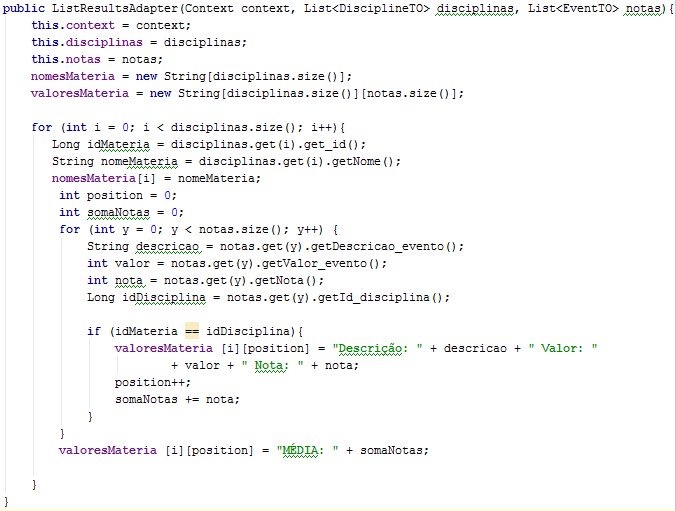
\includegraphics[scale=0.7]{./imagens/2_q_metodologico/4_procedimentos_resultados/42_aplicativo/app8.png}}
		\caption[Adicionando uma dependência ao projeto]{Adicionando uma dependência ao projeto.
		\textbf{Fonte:}Elaborado pelos autores.}
		\label{fig:app9}
	\end{figure}
	
	\par Na tela em que foi aberta localizou-se a biblioteca GSON com o endereço da
Google, logo após selecionou-a e clicou no botão Ok para adicioná-la, como
apresenta a Figura \ref{fig:app10}.
	
	\begin{figure}[h!] 
		\centerline{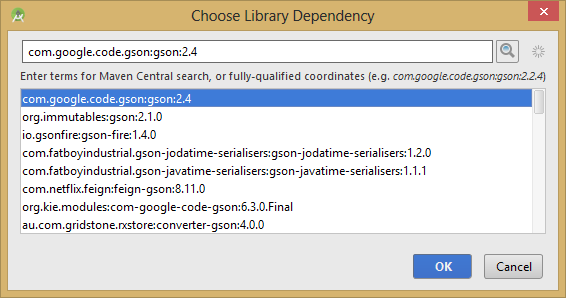
\includegraphics[scale=0.7]{./imagens/2_q_metodologico/4_procedimentos_resultados/42_aplicativo/app9.png}}
		\caption[Adicionando a biblioteca GSON ao projeto]{Adicionando a biblioteca GSON ao projeto.
		\textbf{Fonte:}Elaborado pelos autores.}
		\label{fig:app10}
	\end{figure}
	
	\par Na Figura \ref{fig:app11}, é mostrado o código onde é utilizado a
	biblioteca GSON. O sistema lê os dados vindos em JSON e envia para o GSON que faz a conversão dos
dados no formato da classe \texttt{EventTO}.

	\begin{figure}[h!] 
		\begin{lstlisting}[style=custom_JAVA]
			...
	Reader reader = new InputStreamReader(content);
    Gson gson = new Gson();
    retornoEventos = gson.fromJson(reader, Events.class);
			...
\end{lstlisting}
		\caption[Usando GSON para conversão dos dados]{Usando GSON para conversão dos dados.
		\textbf{Fonte:}Elaborado pelos autores.}
		\label{fig:app11}
	\end{figure}
	
	\par Depois, fez-se necessário construir uma classe que fizesse o gerenciamento
dos dados vindos do banco de dados com a interface que listará as informações
aos usuários. Essa classe recebeu o nome de \texttt{ListResultsAdapter} e
estende da classe nativa do Android denominada
\texttt{BaseExpandableListAdapter}.

	\par Nesta classe foi criado um construtor que recebe a lista de disciplinas
cursadas pelo aluno e uma lista com as notas de cada matéria. Os nomes das
disciplinas foram inseridos em um \textit{array} de \textit{Strings}, já as
notas foram inseridas em uma matriz. Este procedimento foi necessário devido a
estrutura dos métodos \texttt{getGroupView()} e \texttt{getChildView()}
responsável por apresentar na tela do dispositivo os nomes das disciplinas e as
notas das matérias respectivamente.  A Figura \ref{fig:app12} apresenta o
construtor da classe \texttt{ListResultsAdapter}.

	\begin{figure}[h!] 
		\begin{lstlisting}[style=custom_JAVA]
public ListResultsAdapter(Context context, List<DisciplineTO> disciplines, List<EventTO> results){
    this.context = context;
    this.disciplines = disciplines;
    this.results = results;
    namesDisciplines = new String[disciplines.size()];
    EventsDisciplines = new String[disciplines.size()][results.size()];

    for (int i = 0; i < disciplines.size(); i++){
        Long idDiscipline = disciplines.get(i).get_id();
        String nameDiscipline = disciplines.get(i).getName();
        namesDisciplines[i] = nameDiscipline;
        int position = 0;
        int totalResults = 0;
        for (int y = 0; y < results.size(); y++) {
            String description = results.get(y).getDescription_event();
            int value = results.get(y).getValue_event();
            int result = results.get(y).getResult();
            Long disciplineId = results.get(y).getId_discipline();

            if (idDiscipline == disciplineId){
                EventsDisciplines [i][position] = "Descricao: " + description +
                " Valor: " + value + " Nota: " + result;
                position++;
                totalResults += result;
            }
        }
        EventsDisciplines [i][position] = "SOMA DAS NOTAS: " + totalResults;
    }
}
\end{lstlisting}
		\caption[Construtor da classe ListResultsAdapter]{Construtor da classe ListResultsAdapter.
		\textbf{Fonte:}Elaborado pelos autores.}
		\label{fig:app12}
	\end{figure}

	\par Após adicionado os dados no \textit{array} e na matriz é preciso exibí-los
ao estudante. Na Figura \ref{fig:app13}, pode se ver o método \texttt{getGroupView()}
criando um \textit{widget} do tipo \textit{textView}  e inserindo nele o nome
da matéria, os espaçamentos, o tamanho da fonte e informando que as palavras
serão escritos em negrito.

	\begin{figure}[h!] 
		\begin{lstlisting}[style=custom_JAVA]
@Override
    public View getGroupView(int groupPosition, boolean isExpanded,
                             View convertView, ViewGroup parent) {

        TextView textViewDiscipline = new TextView(context);
        textViewDiscipline.setText(namesDisciplines[groupPosition]);
        textViewDiscipline.setPadding(40, 10, 0, 10);
        textViewDiscipline.setTextSize(20);
        textViewDiscipline.setTypeface(null, Typeface.BOLD);

        return textViewDiscipline;
    }
\end{lstlisting}
		\caption[Método getGroupView()]{Método \texttt{getGroupView()}.
		\textbf{Fonte:}Elaborado pelos autores.}
		\label{fig:app13}
	\end{figure}
	
	\pagebreak

	\par O método \texttt{getChildView()} segue a mesma lógica do método
\texttt{getGroupView()}, como ilustra a Fugura \ref{fig:app14}.

	\begin{figure}[h!] 
		\begin{lstlisting}[style=custom_JAVA]
@Override
    public View getChildView(int groupPosition, int childPosition,
                             boolean isLastChild, View convertView, ViewGroup parent) {

        TextView textViewSubList = new TextView(context);
        textViewSubList.setText(EventsDisciplines[groupPosition][childPosition]);
        textViewSubList.setPadding(10, 10, 10, 5);
        textViewSubList.setTextSize(15);

        return textViewSubList;
    }
\end{lstlisting}
		\caption[Método getChildView()]{Método \texttt{getChildView()}.
		\textbf{Fonte:}Elaborado pelos autores.}
		\label{fig:app14}
	\end{figure}
	
	\par O próximo passo, foi criação de uma \textit{activity} do tipo
\textit{blank activity} com finalidade de listar as notas. Ao criá-la com o
nome de \texttt{ListResultsActivity}, o Android Studio gerou dentro da pasta
\textit{layout} o arquivo XML referente a ela, chamado de
\texttt{activity\_list\_results.xml}. Neste, foi inserido apenas o
\textit{widget} \texttt{expandableListView}, que está incumbido de apresentar
a lista de disciplinas cujo o discente está cursando e ao clicar em alguma
dessas matérias serão apresentadas as notas referentes às atividades
realizadas nesta disciplina. Na Figura \ref{fig:app15} é possível ver o código XML de uma
lista do tipo \texttt{expandableListView}.

	\begin{figure}[h!] 
		\begin{lstlisting}[style=custom_XML]
<RelativeLayout 
	xmlns:android="http://schemas.android.com/apk/res/android"
    xmlns:tools="http://schemas.android.com/tools" 
    android:layout_width="match_parent"
    android:layout_height="match_parent" 
    android:paddingLeft="@dimen/activity_horizontal_margin"
    android:paddingRight="@dimen/activity_horizontal_margin"
    android:paddingTop="@dimen/activity_vertical_margin"
    android:paddingBottom="@dimen/activity_vertical_margin"
    android:theme="@style/AppTheme"
    tools:context="univas.edu.com.university.ListResultsActivity">

    <ExpandableListView
        android:layout_width="wrap_content"
        android:layout_height="wrap_content"
        android:id="@+id/expandableListView2"
        android:divider="#FFFFFF"
        android:dividerHeight="1dp"
        android:layout_alignParentBottom="true"
        android:layout_alignParentStart="true"
        android:layout_alignParentTop="true" />

</RelativeLayout>
\end{lstlisting}
		\caption[Código XML do layout que apresentará a lista de notas]{Código XML do
		\textit{layout} que apresentará a lista de notas.
		\textbf{Fonte:}Elaborado pelos autores.}
		\label{fig:app15}
	\end{figure}
	
	\pagebreak
	
	\par Na classe \texttt{ListResultsActivity}, é preciso informar o layout a ser
chamado através do método \texttt{setContentView()}. Além disso, também foi
necessário passar para a classe \texttt{ListResultsAdapter} a lista de
disciplinas que o discente está cursando e a lista com as notas referentes a
cada matéria vindas do banco de dados. Na Figura \ref{fig:app16} é exibido o
método \texttt{onCreate()} da classe \texttt{ListResultsActivity}. 
	
	
	\begin{figure}[h!] 
		\begin{lstlisting}[style=custom_JAVA]
@Override
protected void onCreate(Bundle savedInstanceState) {
    super.onCreate(savedInstanceState);
    setContentView(R.layout.activity_list_results);
    helper = new DatabaseHelper(this);

    execute = new DatabaseExecute(helper);

    ExpandableListView listView = 
    		(ExpandableListView) findViewById(R.id.expandableListView2);
    listView.setAdapter(
    	new ListResultsAdapter(
        	this, 
        	execute.getDisciplines(),
        	execute.getResults())
    	); 
}
\end{lstlisting}
		\caption[ Método onCreate() da classe ListResultsActivity]{ Método
		\texttt{onCreate()} da classe \texttt{ListResultsActivity}.
		\textbf{Fonte:}Elaborado pelos autores.}
		\label{fig:app16}
	\end{figure}

	\par Estes procedimentos que foram realizados para as classes
\texttt{ListResultsActivity} e \texttt{ListResultsAdapter}, eram necessários
para se apresentar as notas dos exercícios resolvidos. Desta mesma forma foi
preciso criar uma \textit{activity} e um \texttt{adapter} tanto para faltas
quanto para provas agendadas seguindo a mesma lógica.

	\par No momento em que algum professor lançar notas, faltas ou provas agendadas
no portal do aluno, é indispensável notificar o estudante. Com esse intuito
desenvolveu-se uma classe chamada de \texttt{GcmIntentServiceUnivas} que
estende \texttt{IntentService}, que recebe a mensagem vinda do GCM.

	\par Esta classe recebe os dados em formato JSON, por isso ela transfere estas
informações para o método \texttt{getJsonEvents()} da classe
\texttt{HttpUtilUnivas}, o qual será responsável por ler os dados e realizar os
procedimentos de gravação no banco de dados.

	\par Ao salvar o evento é chamado o método \texttt{sendNotification()}, que
receberá um objeto da classe \texttt{EventTO}. Ele realiza uma análise do tipo
de evento, para saber qual activity deve ser executada quando o usuário clicar
na notificação. Logo após adicionado os atributos da notificação, como o ícone,
o título e a mensagem, a notificação é exibida ao usuário. Na Figura
\ref{fig:app17} é visível o método \texttt{sendNotification()}.

	\begin{figure}[h!] 
		%\begin{lstlisting}[style=custom_JAVA]
private void sendNotification(EventTO to) {
        String msg;
        DisciplineTO disciplineTO = execute.getDispline(to.getId_discipline());
        String nameDispline = disciplineTO.getName();
        mNotificationManager = (NotificationManager)
                this.getSystemService(Context.NOTIFICATION_SERVICE);
        PendingIntent contentIntent;
        if(to.getType_event().equals("PROVA_AGENDADA")){
            List<String> data = new ArrayList<String>();
            data.add(nameDispline);
            data.add(to.getDescription_event());
            data.add(String.valueOf(to.getValue_event()));
            data.add(to.getDate_event());
            Intent intent = new Intent(this, NotificationAgendasActivity.class);
            intent.putExtra("dados", (ArrayList<String>)data);
            contentIntent = PendingIntent.getActivity(this, 0, intent, 0);

            msg = "Prova agendada dia" + to.getDate_event();
        }else{
            if(to.getType_event().equals("FALTAS")){
                List<String> data = new ArrayList<String>();
                data.add(nameDispline);
                data.add(to.getDate_event());
                data.add(String.valueOf(to.getValue_event()));
                Intent intent = new Intent(this, NotificationFoulsActivity.class);
                intent.putExtra("dados", (ArrayList<String>)data);

                contentIntent = PendingIntent.getActivity(this, 0, intent, 0);

                msg = to.getValue_event() + " falta(s) recebidas";
            }else{
                List<String> data = new ArrayList<String>();
                data.add(nameDispline);
                data.add(to.getDescription_event());
                data.add(String.valueOf(to.getValue_event()));
                data.add(String.valueOf(to.getResult()));
                Intent intent = new Intent(this, NotificationResultsActivity.class);
                intent.putExtra("dados", (ArrayList<String>)data);

                contentIntent = PendingIntent.getActivity(this, 0, intent, 0);
               msg = "Nova nota " + to.getResult();
            }
        }

        Uri soundUri = RingtoneManager.getDefaultUri(RingtoneManager.TYPE_NOTIFICATION);

        NotificationCompat.Builder mBuilder = new NotificationCompat.Builder(this)
        .setSmallIcon(R.drawable.notification_univas)
        .setContentTitle("Univas informa")
        .setAutoCancel(true)
        .setStyle(new NotificationCompat.BigTextStyle()
        .bigText(msg))
        .setContentText(msg)
        .setSound(soundUri);
        
        Vibrator vibrator = (Vibrator) getSystemService(Context.VIBRATOR_SERVICE);
        long milliseconds = 30;
        vibrator.vibrate(milliseconds);

        mBuilder.setContentIntent(contentIntent);
        mNotificationManager.notify(NOTIFICATION_ID, mBuilder.build());
}
\end{lstlisting}
		\caption[Método sendNotification()]{ Método \texttt{sendNotification()}.
		\textbf{Fonte:}Elaborado pelos autores.}
		\label{fig:app17}
	\end{figure}
	

	\par A notificação acontece toda vez que o GCM envia uma informação ao
dispositivo. Para tratar essas ocorrências foi projetada uma classe para ser o
\texttt{BroadcastReceiver} chamada de \texttt{GcmBroadcastReceiverUnivas}. Ela
estende da classe \texttt{WakefulBroadcastReceiver} nativa do Android e possui
apenas um método chamado de \texttt{onReceive()}, o qual receberá a
\textit{intent} a ser chamada quando chegar algum dado do GCM. Na Figura
\ref{fig:app18}, vê-se a classe \texttt{GcmBroadcastReceiverUnivas}, que
através do método \texttt{onReceive()} inicializará a classe
\texttt{GcmIntentServiceUnivas}.

	\begin{figure}[h!] 
		\begin{lstlisting}[style=custom_JAVA]
public class GcmBroadcastReceiverUnivas extends WakefulBroadcastReceiver {

    @Override
    public void onReceive(Context context, Intent intent) {
        ComponentName comp = new ComponentName(context.getPackageName(),  GcmIntentServiceUnivas.class.getName());
        startWakefulService(context, (intent.setComponent(comp)));
        setResultCode(Activity.RESULT_OK);
    }
}
\end{lstlisting}
		\caption[Classe GcmBroadcastReceiverUnivas]{Classe
		\texttt{GcmBroadcastReceiverUnivas}.
		\textbf{Fonte:}Elaborado pelos autores.}
		\label{fig:app18}
	\end{figure}
		
	\par No entanto para configurar esta classe como um \texttt{BroadcastReceiver},
foi preciso adicioná-la na tag \texttt{<receiver>} do arquivo
\texttt{AndroidManifest.XML}, como mostra a Figura \ref{fig:app19}.

	\begin{figure}[h!] 
		\begin{lstlisting}[style=custom_XML]
<receiver
	android:name=".model.GcmBroadcastReceiverUnivas"
	android:permission="com.google.android.c2dm.permission.SEND" >
		<intent-filter>
		    <action android:name="com.google.android.c2dm.intent.RECEIVE" />
		    <category android:name="univas.edu.com.university.model" />
		</intent-filter>
</receiver>
\end{lstlisting}
		\caption[Configuração do BroadcastReceiver no
		AndroidManifest.XML]{Configuração do \texttt{BroadcastReceiver} no
		\texttt{AndroidManifest.XML}.
		\textbf{Fonte:}Elaborado pelos autores.}
		\label{fig:app19}
	\end{figure}

	\par Por fim, foi construída uma classe chamada de \texttt{GcmControllerUnivas}
que tem por objetivo configurar o dispositivo para trabalhar com o GCM.

	\par Nesta classe existe um método denominado \texttt{checkPlayServices()} como
intuito de verificar se o dispositivo possui os requisitos necessários para o
GCM. Na Figura \ref{fig:app20}, é apresentado o método checkPlayServices().

	\begin{figure}[h!] 
		\begin{lstlisting}[style=custom_JAVA]
public boolean checkPlayServices() {

        int resultCode = GooglePlayServicesUtil.isGooglePlayServicesAvailable(context);

        if (resultCode != ConnectionResult.SUCCESS) {

            if (GooglePlayServicesUtil.isUserRecoverableError(resultCode)) {

                GooglePlayServicesUtil.getErrorDialog(
                	resultCode, 
                	new MainActivity(), 
                	PLAY_SERVICES_RESOLUTION_REQUEST
                ).show();

            } else {
                Log.i(TAG, "Este dispositivo nao suporta o GCM.");
            }
            return false;
        }
        return true;
    }
\end{lstlisting}
		\caption[Método checkPlayServices()]{Método \texttt{checkPlayServices()}.
		\textbf{Fonte:}Elaborado pelos autores.}
		\label{fig:app20}
	\end{figure}
	
	\par Logo após é chamado o método \texttt{getRegistrationId()}, que é incumbido
de retornar o \textit{Registration} ID. Na Figura \ref{fig:app21} é possível ver
este método, no entanto, se o registro retornado for nulo, isso significa que o
aparelho não está cadastrado nos servidores da Google, então é executado o
método \texttt{registerInBackground()} que fará esse cadastro, como demostra a
Figura \ref{fig:app22}.

	\begin{figure}[h!] 
		\begin{lstlisting}[style=custom_JAVA]
private String getRegistrationId(Context context) {

        final SharedPreferences prefs = getGcmPreferences(context);

        String registrationId = prefs.getString(PROPERTY_REG_ID, "");
        if (registrationId.isEmpty()) {
            Log.i(TAG, "Falha ao registrar.");
            return "";
        }
  
        int registeredVersion = prefs.getInt(PROPERTY_APP_VERSION, Integer.MIN_VALUE);
        int currentVersion = getAppVersion(context);
        if (registeredVersion != currentVersion) {
            Log.i(TAG, "Versao alterada do aplicativo.");
            return "";
        }
        return ;
}
\end{lstlisting}
		\caption[Método getRegistrationId()]{Método \texttt{getRegistrationId()}.
		\textbf{Fonte:}Elaborado pelos autores.}
		\label{fig:app21}
	\end{figure}
	
	\begin{figure}[h!] 
		\begin{lstlisting}[style=custom_JAVA]
private void registerInBackground() {

        new AsyncTask<Void, Void, String>() {
            @Override
            protected String doInBackground(Void... params) {
                String msg = "";
                try {
                    if (gcm == null) {
                        gcm = GoogleCloudMessaging.getInstance(context);
                    }
                    regid = gcm.register(SENDER_ID);
                    msg = "Dispositivo registrado, registro ID=" + regid;

                    sendRegistrationIdToBackend(regid);

                    storeRegistrationId(context, regid);
                } catch (IOException ex) {
                    msg = "Error :" + ex.getMessage();
                }
                return msg;
            }

            @Override
            protected void onPostExecute(String msg) {
                Toast.makeText(new MainActivity(), msg, Toast.LENGTH_SHORT).show();
            }
        }.execute(null, null, null);
    }
\end{lstlisting}
		\caption[Método registerInBackground()]{Método
		\texttt{registerInBackground()}.
		\textbf{Fonte:}Elaborado pelos autores.}
		\label{fig:app22}
	\end{figure}
	
	\par Desta forma, quando o \textit{web service} envia uma informação ao GCM, o
\textit{Registration} ID é transmitido junto aos dados, gerado pelo método
\texttt{registerInBackground()}, possibilitando ao serviço da Google
identificar a qual dispositivo deve conduzir a mensagem.
	
			%web service
			\subsection{\textit{Web service}}	
				\subsection{\textit{Webservice}}

\par No que diz respeito à contrução do \textit{webservice}, foi necessária a
instalação e configuração de um ambiente de desenvolvimento compatível com as
necessidades apresentadas pelo \textit{software} e que foram levantadas através
dos requisitos. Foi instalado o \textit{Servlet Container Apache Tomcat} em sua
versão de número 7. O \textit{Servlet Container} foi instalado para que o
\textit{Web Service} pudesse fornecer os serviços necessários para o consumo de
dados do Aplicativo \textit{Android}, haja vista que \textit{Apache tomcat} faz
uso amplo do protocolo HTTP\footnote{HTTP - Hypertext Transfer Protocol} e da
plataforma \textit{Java} de desenvolvimento.
			
		\par Para armazenar os dados gerados e/ou recebidos, foi necessário fazer a
	intalação do Sistema Gerenciador de Banco de Dados(SGBD) \textit{PostGreSql} na
	sua versão de número 9.2. Através de um levantamento de requisitos parciais e das
	reuniões entre os participantes foi possível construir um Diagrama de Entidade
	e Relacionamento, no qual ficou definida a estrutura do banco de dados da
	aplicação. A Figura \ref{fig:qm9} mostra o Diagrama de Entidade e
	Relacionamento concebido para esta pesquisa.

		\begin{figure}[h!]
			\centerline{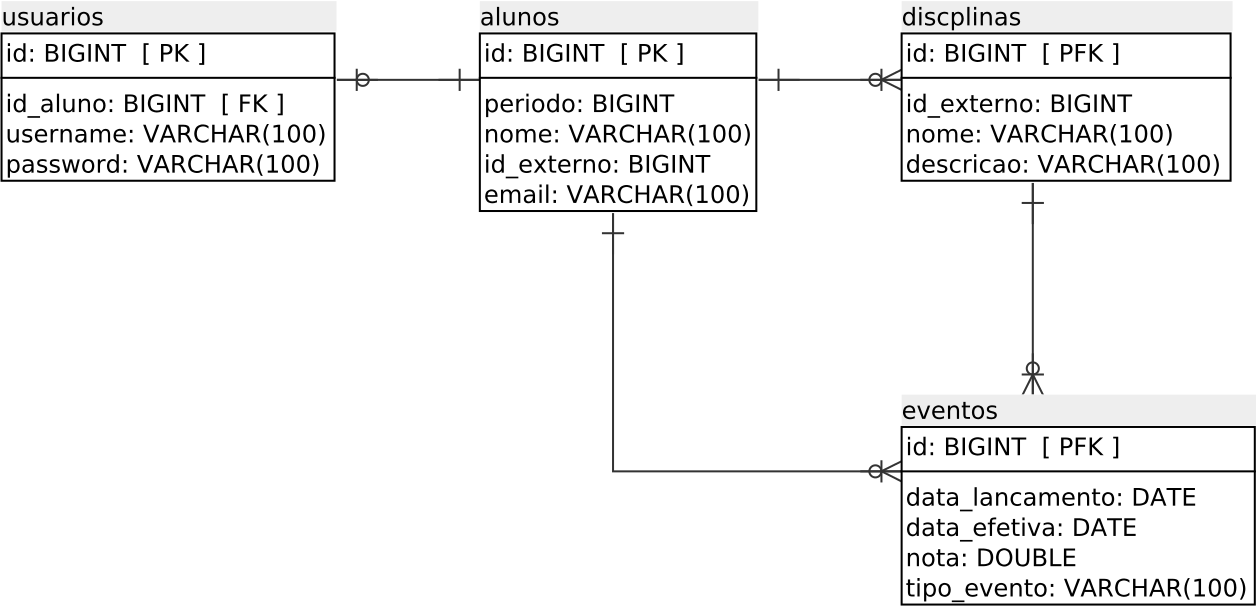
\includegraphics[scale=0.4]{./imagens/2_q_metodologico/qm9.png}}
			\caption[Diagrama de Entidade e Relacionamento]{Diagrama de Entidade e
			Relacionamento.
			\textbf{Fonte:}Elaborado pelos autores.}
			\label{fig:qm9}
		\end{figure}
\pagebreak
		\par Fazendo uso desse diagrama foi possível criar todas as classes 
	\textit{Java} que representam as entidades do mapeamento objeto-relacional. 
	Essas classes foram criadas fazendo uso de anotações próprias do
	\textit{Hibernate}, que é um \textit{framework} que implementa a especificação
	JPA\footnote{JPA - \textit{Java Persistense API}}. Essas classes fazem parte
	dos mecanismos de persistêcia de dados e são simplesmente t ou seja, objetos
	simples que contêm somente atributos privados e os métodos \textit{getters} e
	\textit{setters} que servem apenas para encapsular estes atributos. Uma das
	classes criadas, foi a classe \texttt{Aluno.java} que representa a tabela
	\texttt{alunos} no banco de dados e está representada na Figura
	\ref{fig:qm10}.%mudar para figura
	
		\begin{figure}[h!]
			\centerline{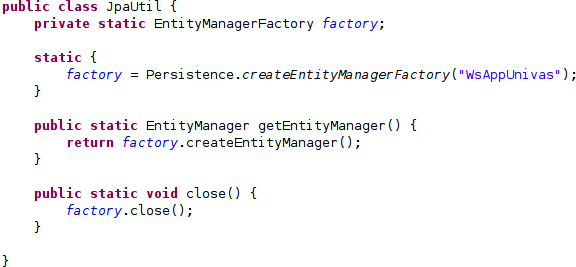
\includegraphics[scale=0.7]{./imagens/2_q_metodologico/qm10.png}}
			\caption[Classe \texttt{Aluno}]{Classe \texttt{Aluno}.
			\textbf{Fonte:}Elaborado pelos autores.}
			\label{fig:qm10} 
		\end{figure}
		
		\pagebreak
		
		\par Foram criadas outras classes \textit{Java} com a mesma finalidade da
	anterior, porém com pequenas diferenças no que diz respeito à atributos,
	metodos e anotações. Estas classes representam, de maneira individual, as
	tabelas no banco de dados. Certos atributos dessas classes têm por finalidade
	representar as colunas de cada tabela. Já os atributos que armazenam instâncias
	de outras classes ou até mesmo conjuntos (coleções) de instâncias representam os
	relacionamentos entre as tabelas. E por fim, para cada classe que representa uma
	entidade, foi necessário implementar os métodos \texttt{hashCode} e
	\texttt{equals}, para que estas pudessem facilmente ser comparadas e
	diferenciadas em relação aos seus valores, haja visto que cada instância
	destas classes representa um registro no banco de dados.
		
		\par Em seguida à criação das entidades, foi necessário configurar o arquivo
	\texttt{persistence.xml} que fica dentro do \textit{classpath} do projeto
	\textit{Java} ou seja, dentro da mesma pasta onde estão contidos pacotes do
	projeto. Este arquivo é extremamente importante, pois é nele que estão todas
	as configurações relativas à conexão com o banco de dados, configurações
	referentes ao Dialeto SQL que vai ser usado para as consultas e configurações
	referentes ao \textit{persistence unit} que é o conjunto de classes mapeadas
	para o banco de dados.	O arquivo \texttt{persistence.xml} está exposto no
	código \ref{fig:qm11}.
	
 		\begin{figure}[h!]
			\centerline{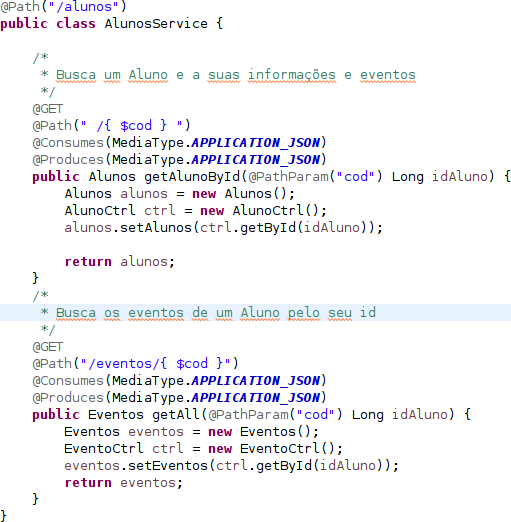
\includegraphics[scale=0.6]{./imagens/2_q_metodologico/qm11.png}}
			\caption[Arquivo \texttt{persistence.xml}]{Arquivo \texttt{persistence.xml}.
			\textbf{Fonte:}Elaborado pelos autores.}
			\label{fig:qm11}
		\end{figure}
		
			\par Em seguida à confecção do \texttt{persistence.xml} foi criada a
		classe \texttt{JpaUtil} que está representada na Figura \ref{fig:qm12}.
		Esta classe é responsável por criar uma \texttt{EntityManagerFactory} que é
		uma  fábrica de instâncias de \texttt{EntityManager} que nada mais é que um
		\textit{persistence unit} ou unidade de persistência. Essa classe tem a
		responsabilidade de prover um modo de comunicação entre a aplicação e o banco
		de dados. No entanto a classe \texttt{JpaUtil} cria uma única instância de
		\texttt{EntityManagerFactory}, que é responsável por disponibilizar e
		gerenciar as instâncias de \texttt{EntityManager} de acordo com a necessidade
		da aplicação.
		
		\pagebreak
		\begin{figure}[h!]
			\centerline{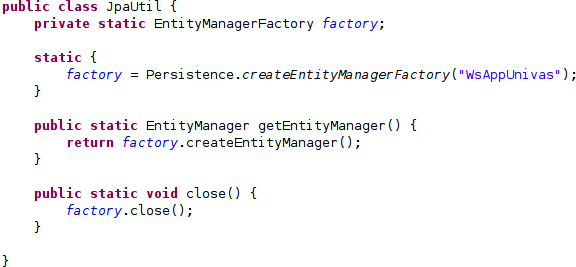
\includegraphics[scale=0.7]{./imagens/2_q_metodologico/qm12.png}}
			\caption[Classe \texttt{JpaUtil}]{Classe \texttt{JpaUtil}.
			\textbf{Fonte:}Elaborado pelos autores.}
			\label{fig:qm12}
		\end{figure}
		
	\par Em seguida à construção das classes que fazem a parte da persistência de
dados, foi desenvolvido a parte de disponibilização de serviços
\textit{RESTful}, fazendo uso do \textit{framework} \textit{Jersey}. Com isso
pode-se construir a classe que representa o primeiro serviço do
\textit{webservice}, que é a classe \texttt{Alunos}. Essa classe representa um
contexto REST, e portanto, dispõe de alguns recursos. Esses recursos fazem a
recuperação e a transmissão dos dados do \textit{webservice} para o aplicativo
\textit{Android}. Essa classe e seus respectivos métodos  estão representada na
Figura \ref{fig:qm13}.

		\begin{figure}[h!]
			\centerline{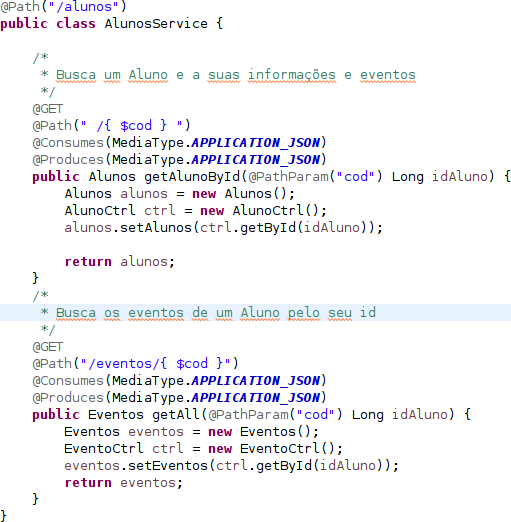
\includegraphics[scale=0.7]{./imagens/2_q_metodologico/qm13.png}}
			\caption[Classe \texttt{AlunosService}]{Classe \texttt{AlunosService}.
			\textbf{Fonte:}Elaborado pelos autores.}
			\label{fig:qm13}
		\end{figure}
		
		\par O \textit{webservice} pode fazer a busca de alunos pelo \texttt{id}
passado ou retornar uma coleção de eventos vinculados a um alunos, dependendo
do recurso acessado. Os tipos de dados que o \textit{webservice} consome e
retorna é o JSON\footnote{JSON - \textit{Javascript Object Notation}}. Não foi
necessário fazer nenhuma implementação adicional relativa a este formato, pois
o próprio \textit{framework Jersey} faz o tratamento e a conversão dos tipos de
entrada e saída de dados. No caso do saída de dados, faz a conversão de objetos 
\textit{Java} para JSON. E no caso de entrada tranforma um JSON em objeto
\textit{Java} já conhecido pelo \textit{webservice}. Com isso concluiu-se o
desenvolvimento do \textit{webservice} que fornece os dados para o aplicativo.

	\par Para que fosse possível transmitir dados para o aplicativo, era
necessário receber as informações do sistema acadêmico da referida instituição,
haja vista que o \textit{web service} é independente do mesmo. Para esse
propósito é necessário  contruir um módulo que faça a importação dos dados
necessários para a base de dados do \textit{web service}. Este por sua vez
terá a responsabilidade de fazer a importação dos dados periodicamente, e
ainda tratar os tipos de dados recebidos para tipos aplicáveis ao banco de
dados local. Além disso é preciso notificar o módulo responsável por invocar
o serviço \textit{Google Cloud Messaging} para que os dispositivos dos alunos
aos quais houveram atualizações nos dados, fossem notificados e fizessem acesso
ao \textit{web service} para solicitar esses dados atualizados.

	\par Os procedimentos acima citados foram os passos até agora realizados com o
propósito de se alcançar os resultados esperados para essa pesquisa.
	
						%Ambiente de desenvolvimento
						\subsubsection{Montagem do Ambiente de Desenvolvimento}
							%\subsubsection{Montagem do Ambiente de Desenvolvimento}
	
	\par No que diz respeito à contrução do \textit{web service}, foi necessária a
instalação e configuração de um ambiente de desenvolvimento compatível com as
necessidades apresentadas pelo software.

	\par A princípio foi instalado o \textit{Servlet Container} Apache Tomcat em
sua versão de número {7}. Este \textit{Servlet Container} foi instalado pois
implementa a API da especificação \textit{Servlets} {3.0} do Java. Isso era
necessário pelo fato que o \textit{framework} Jersey usa \textit{servlets} para
disponibilizar serviços REST. Além disso o Apache Tomcat foi escolhido, para
que o \textit{web service} pudesse fornecer os serviços necessários para o
consumo do aplicativo, na arquitetura REST, que sugere o uso do protocolo
HTTP\footnote{HTTP - Hypertext Transfer Protocol} para troca de mensagens, pois
além da funcionalidade com \textit{Servlets}, o Apache Tomcat também é um
servidor HTTP.
	
	\par O Apache Tomcat foi instalado, por meio do \textit{download} de um
arquivo compactado, de seu site oficial. A instalação consiste apenas
em extrair os dados do arquivo em uma pasta da preferência do desenvolvedor.
Esta abordagem permitiu a integração do Apache Tomcat com a
IDE\footnote{IDE - Integrated Development Environment}
Eclipse, que foi usada para o desenvolvimento. Com isto foi possível controlar
e monitorar, o servidor de aplicações através da IDE. Além da configuração
necessária para integrar o servidor à IDE, nenhuma outra configuração foi
necessária.

	\par Como ferramenta para desenvolvimento, foi usada a IDE Eclipse na versão
{4.4}, que é popularmente conhecida como Luna. O processo de instalação e
configuração da IDE, se assemelha bastante ao processo de instalação do Apache
Tomcat, pois somente é necessário fazer o download do arquivo compactado que é
fornecido na página do projeto, e descompactá-lo no local preferido pelo
desenvolvedor.

	\par Para armazenar os dados gerados e/ou recebidos, foi necessário fazer a
intalação do Sistema Gerenciador de Banco de Dados (SGBD) PostGreSql na sua
versão de número {9.4}. Como está sendo usado um sistema operacional baseado em
GNU/Linux como ambiente de desenvolvimento, o PostGreSql foi instalado através
do gerenciador de pacotes da distribuição.
 
%	\par Foi necessário criar um usuário no SGDB que tivesse permissão suficiente
%apenas para fazer as operações referentes ao banco de dados do \textit{web
%service}, evitando assim a necessidade de se trabalhar diretamente com um
%usuário master do SGBD. Esta medida foi tomada visando a segurança do banco de
%dados, pois com isto foi possível isolar e restringir as responsabilidades
% deste usuário.

	
						%desenvolvimento
						\subsubsection{Desenvolvimento}
							%\subsubsection{Desenvolvimento}

	%01 - Criação do database
	
	\par Com o ambiente de desenvolvimento pronto, começou de fato o
desenvolvimento. Primeiramente foi necessário criar o banco de dados no SGDB.
Este por sua vez foi criado com a ajuda do PgAdmin que é um software gráfico
para administração do SGDB, e que fornece uma interface gráfica de apoio para o
PotgreSql. Para criar era necessário ja estar com o PgAdmin aberto e conectado
a um servidor de banco de dados que neste caso era em servidor local como pode
ser visto na Figura \ref{fig:desws}.

	\begin{figure}[h!]
		\centerline{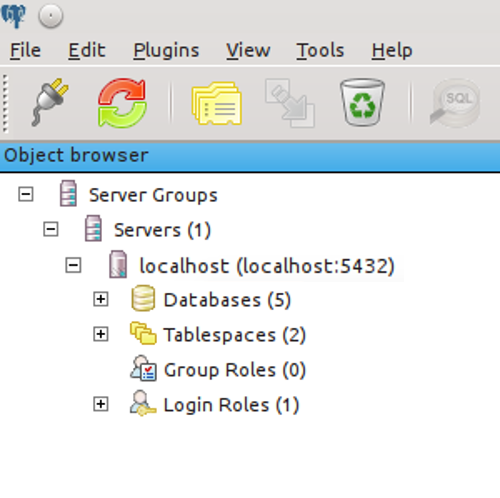
\includegraphics[scale=1]{./imagens/2_q_metodologico/4_procedimentos_resultados/43_webservice/432_desenvolvimento/desws.png}}
		\caption[Servidor de banco de dados local no PgAdmin]{Servidor de banco de
		dados local no PgAdmin.
			\textbf{Fonte:}Elaborado pelos autores.}
		\label{fig:desws}
	\end{figure}
	
	\pagebreak
	
	\par Para a efetiva criação do banco de dados era necessário clicar com o
botão direito do \textit{mouse}, sobre a opção \textbf{Databases -> New
Database\ldots} no PgAdmin, apresentada na Figura \ref{fig:desws1}.

	\begin{figure}[h!]
		\centerline{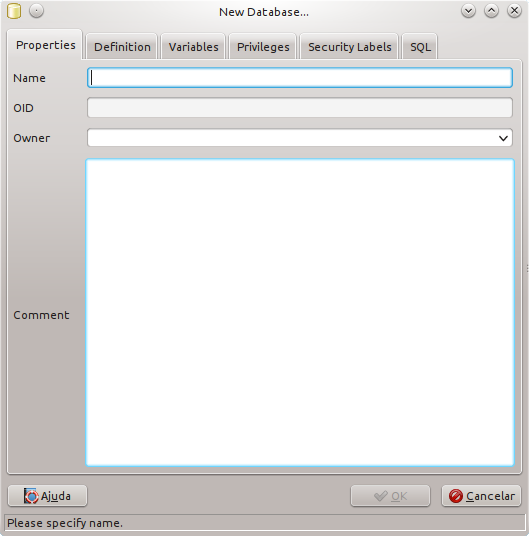
\includegraphics[scale=0.8]{./imagens/2_q_metodologico/4_procedimentos_resultados/43_webservice/432_desenvolvimento/desws1.png}}
		\caption[Opção \textit{New Database\ldots}]{Opção \textit{New Database\ldots}.
			\textbf{Fonte:}Elaborado pelos autores.}
		\label{fig:desws1}
	\end{figure}

	\pagebreak
	
	\par Em seguida foi necessário preencher o dados da janela apresentada, como
está apresentado na Figura \ref{fig:desws2}.
	
	\begin{figure}[h!]
		\centerline{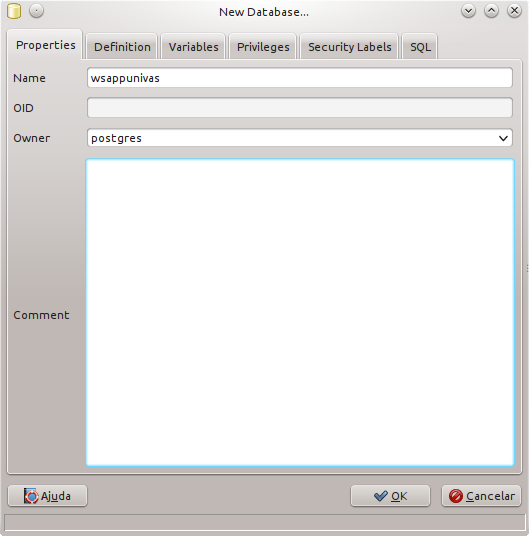
\includegraphics[scale=1]{./imagens/2_q_metodologico/4_procedimentos_resultados/43_webservice/432_desenvolvimento/desws2.png}}
		\caption[Tela \textit{New Database\ldots}]{Tela \textit{New Database\ldots}.
			\textbf{Fonte:}Elaborado pelos autores.}
		\label{fig:desws2}
	\end{figure}
	
	\pagebreak

	\par Como pode ser visto foram preenchidos os campos nome e usuário . O campo
nome se refere ao nome do banco de dados que foi definido com
\texttt{wsappunivas}, e usuário, o responsável pelo banco de dados, que para
este caso foi usuário padrão do SGDB, que é o \texttt{postgres}. Além destas
configurações mais nenhuma foi necessária. O banco de dados foi criado, porém
sua estrutura não foi definida, pois como será visto mais adiante o Hibernate,
possui um mecanismo, que com algumas configurações, permite a estruturação do
banco de dados, de acordo com o mapeamento objeto-relacional e de acordo com a
evolução do projeto. Isto permitirá mudanças na estrutura do banco de dados e
suas tabelas, e até mesmo eventuais correções.
	
	%02 - Início do projeto web no eclipse;
	\par Em seguida foi criado um projeto do tipo Dynamic Web Project no
Eclipse. Para proceder com a criação de um novo projeto deste tipo no Eclipse, é
necessário acessar na IDE, a opção \textbf{File -> New-> Dynamic Web Project}
como pode ser visto na figura \ref{fig:desws3}.

	
	\begin{figure}[h!]
		\centerline{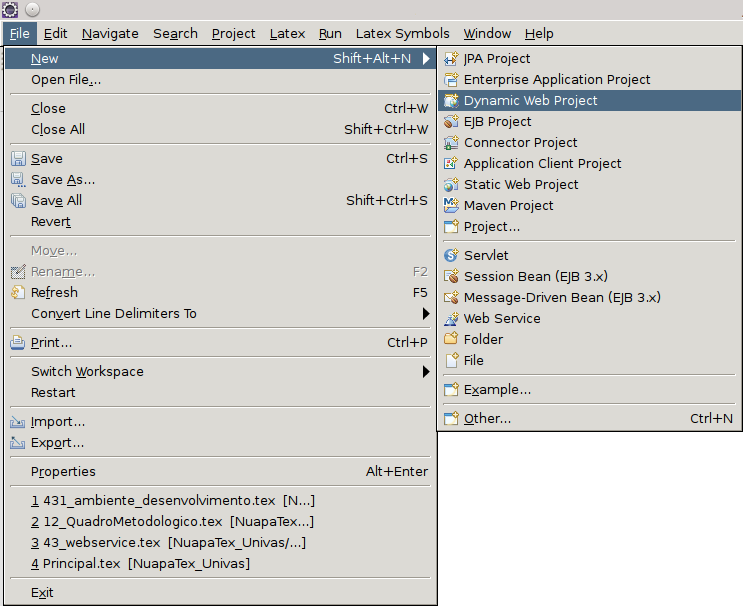
\includegraphics[scale=0.8]{./imagens/2_q_metodologico/4_procedimentos_resultados/43_webservice/432_desenvolvimento/desws3.png}}
		\caption[Tela \textit{New Database\ldots}]{Tela \textit{New Database\ldots}.
			\textbf{Fonte:}Elaborado pelos autores.}
		\label{fig:desws3}
	\end{figure}
	
	\pagebreak
	
 	\par Em seguida foi apresentada uma tela para o preenchimento de alguns dados
 requeridos para a criação do projeto. Destas informações somente foi preenchido
 o nome do projeto. As outras informações continuaram sendo as que vem por
 padrão da IDE. A janela apresentada e as informações preenchidas podem ser
 vistas na Figura \ref{fig:desws4}.

	\begin{figure}[h!]
		\centerline{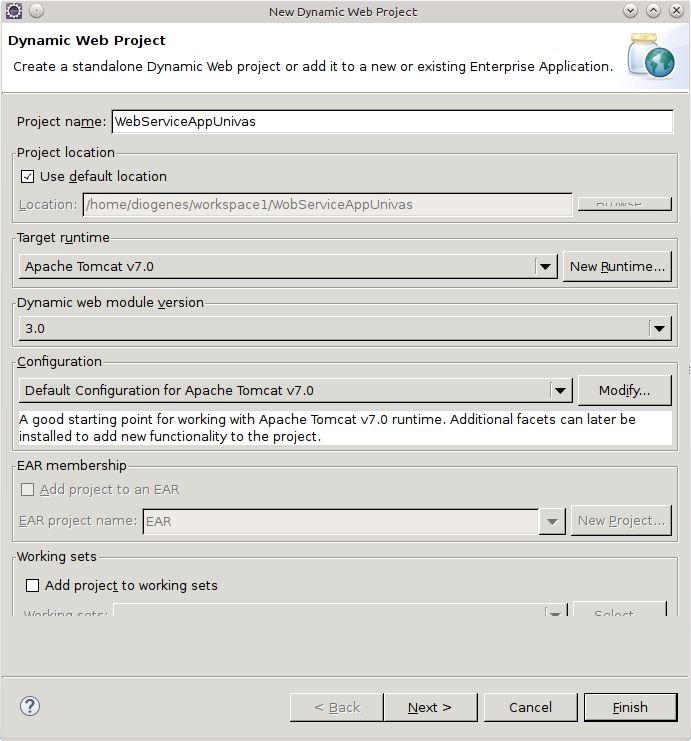
\includegraphics[scale=0.8]{./imagens/2_q_metodologico/4_procedimentos_resultados/43_webservice/432_desenvolvimento/desws4.png}}
		\caption[Tela para criação de um novo projeto no Eclipse]{Tela para criação de um novo projeto no Eclipse.
			\textbf{Fonte:}Elaborado pelos autores.}
		\label{fig:desws4}
	\end{figure}
	
	\pagebreak
	
	
	\par Na próxima janela apresentada, que têm por função configurar a pasta de
códigos do projeto manteve-se a configuração apresentada pela IDE, como mostra
a Figura \ref{fig:desws5}.

	\begin{figure}[h!]
		\centerline{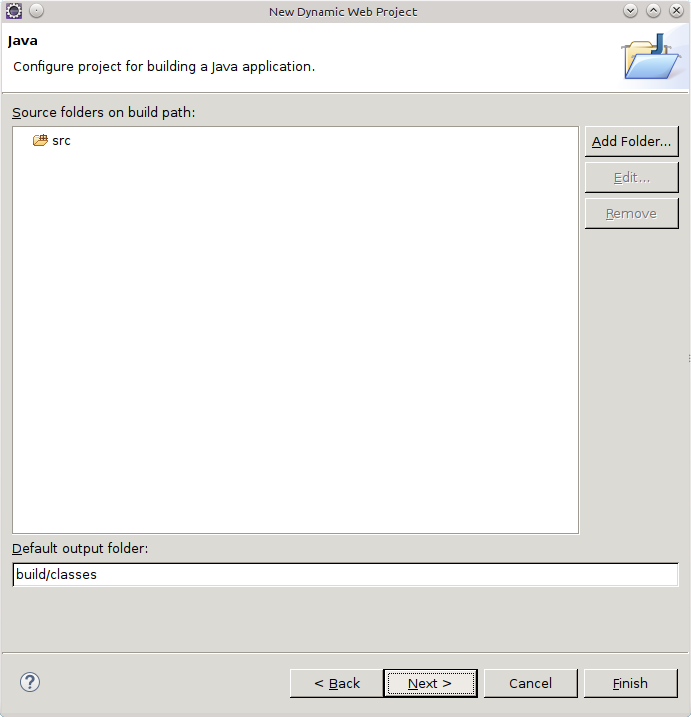
\includegraphics[scale=0.8]{./imagens/2_q_metodologico/4_procedimentos_resultados/43_webservice/432_desenvolvimento/desws5.png}}
		\caption[Tela para criação de um novo projeto no Eclipse]{Tela para criação de um novo projeto no Eclipse.
			\textbf{Fonte:}Elaborado pelos autores.}
		\label{fig:desws5}
	\end{figure}
	
	\pagebreak
	
	\par Na sequencia, na tela que foi apresentada era necessário preencher o
campo \textbf{Context root:} com o contexto principal da aplicação web que
acabou mantendo o próprio nome da aplicação. Além disso foi marcado a opção
\textbf{Generate web.xml deployment descriptor}, para que ao criar o projeto, a
própria IDE criasse o arquivo \texttt{web.xml}, arquivo responsável por algumas
configurações da aplicação web. Esta tela esta apresentada na Figura
\ref{fig:desws6}.

	\begin{figure}[h!]
		\centerline{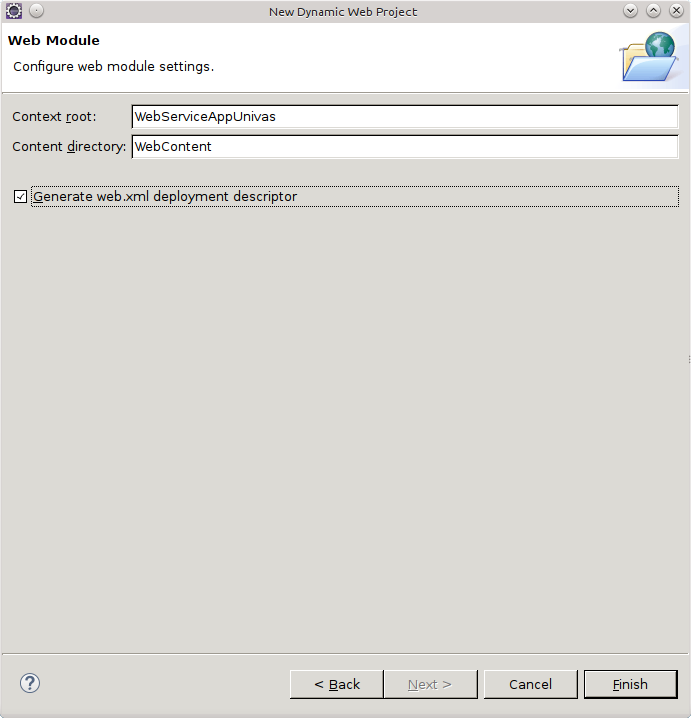
\includegraphics[scale=0.8]{./imagens/2_q_metodologico/4_procedimentos_resultados/43_webservice/432_desenvolvimento/desws6.png}}
		\caption[Tela para criação de um novo projeto no Eclipse]{Tela para criação de um novo projeto no Eclipse.
			\textbf{Fonte:}Elaborado pelos autores.}
		\label{fig:desws6}
	\end{figure}
	
	\pagebreak

	%03 - Mapeamento orm;	
		%	->Criação do pacote

	\par Após este passo foi concluído a criação do projeto, e já era possível
iniciar os trabalhos com a camada de persistência de dados do projeto. Para
este propósito, primeiramente foi criado um pacote, onde ficaram contidas as
classes que representam as entidades do ORM. Para a criação do pacote foi
necessário clicar com o botão direito do mouse sobre o projeto e acessar a opção
\textbf{New -> Package}, como pode ser visto na Figura \ref{fig:desws7}.

	\begin{figure}[h!]
		\centerline{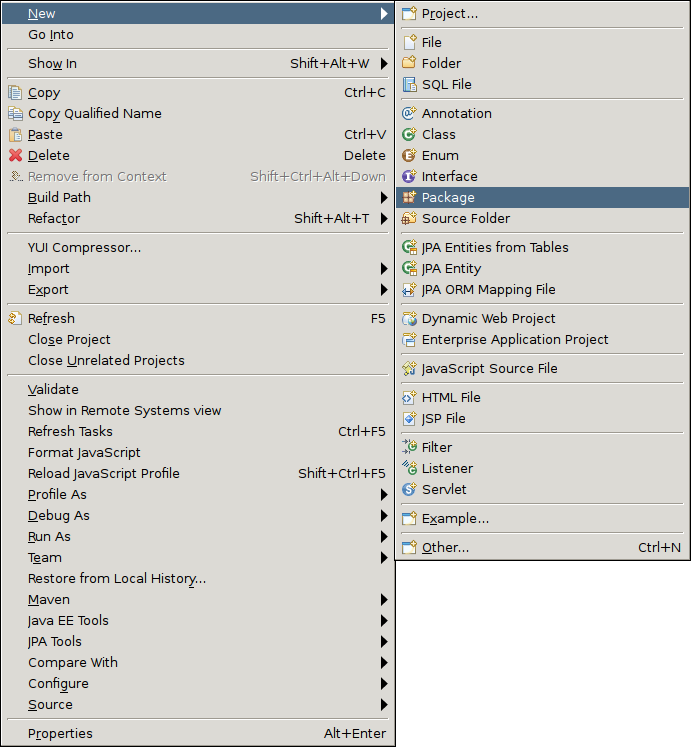
\includegraphics[scale=0.8]{./imagens/2_q_metodologico/4_procedimentos_resultados/43_webservice/432_desenvolvimento/desws7.png}}
		\caption[Tela para criação de um novo projeto no Eclipse]{Tela para criação de um novo projeto no Eclipse.
			\textbf{Fonte:}Elaborado pelos autores.}
		\label{fig:desws7}
	\end{figure}
	
	\pagebreak 
	
	\par Em seguida foi apresentada a janela New Java Package, para a criação de
um novo pacote mostrada na Figura \ref{fig:desws8}. O pacote recebeu o nome de
"\texttt{br.edu.univas.restapiappunivas.model}", pois nele estão contidas as
classes que fazem parte do modelo de negócios da aplicação. Este pacote foi
criado visando a divisão das responsabilidades internas no projeto, além de
contribuir positivamente com a organização do mesmo.

	\begin{figure}[h!]
		\centerline{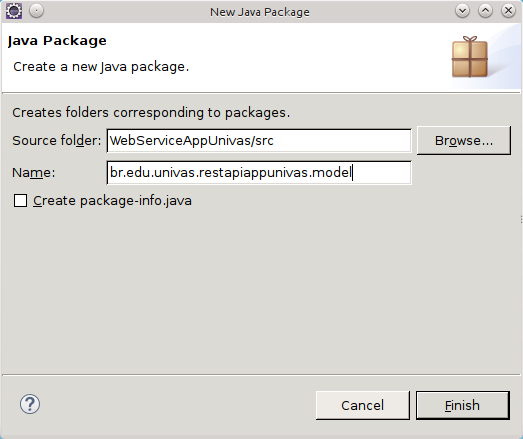
\includegraphics[scale=0.8]{./imagens/2_q_metodologico/4_procedimentos_resultados/43_webservice/432_desenvolvimento/desws8.png}}
		\caption[Tela para criação de um novo projeto no Eclipse]{Tela para criação de um novo projeto no Eclipse.
			\textbf{Fonte:}Elaborado pelos autores.}
		\label{fig:desws8}
	\end{figure}
	
	\pagebreak
		
		%	->Criação das classes
	\par Com este pacote criado, ja era possível criar as classes do ORM. Foi
criada primeiramente a classe \texttt{Student.java}. Para a criação desta classe
foi necesário clicar com o botão direito do \textit{mouse} sobre o projeto e
navegar até a opção \textbf{New -> Class} como pode ser visto na Figura
\ref{fig:desws9}. 

	\begin{figure}[h!]
		\centerline{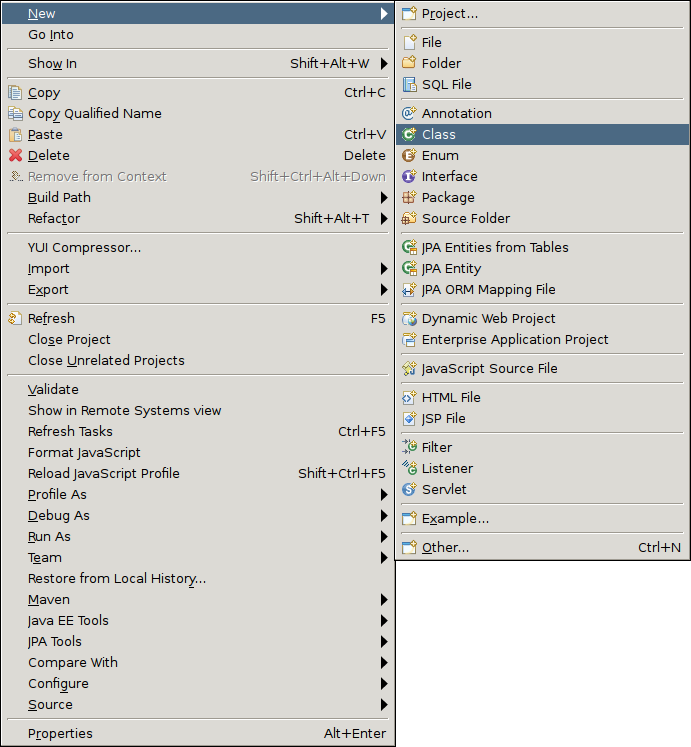
\includegraphics[scale=0.8]{./imagens/2_q_metodologico/4_procedimentos_resultados/43_webservice/432_desenvolvimento/desws9.png}}
		\caption[Sem legenda]{Sem legenda.
			\textbf{Fonte:}Elaborado pelos autores.}
		\label{fig:desws9}
	\end{figure}
	
	\pagebreak


	\par Em seguida foi apresentada uma janela chamada New Java Class. Nesta
janela somente foi necessário preencher o campo \textbf{Name:} que representa o
nome da classe que está sendo criada.
	
	
	
	 \begin{figure}[h!]
		\centerline{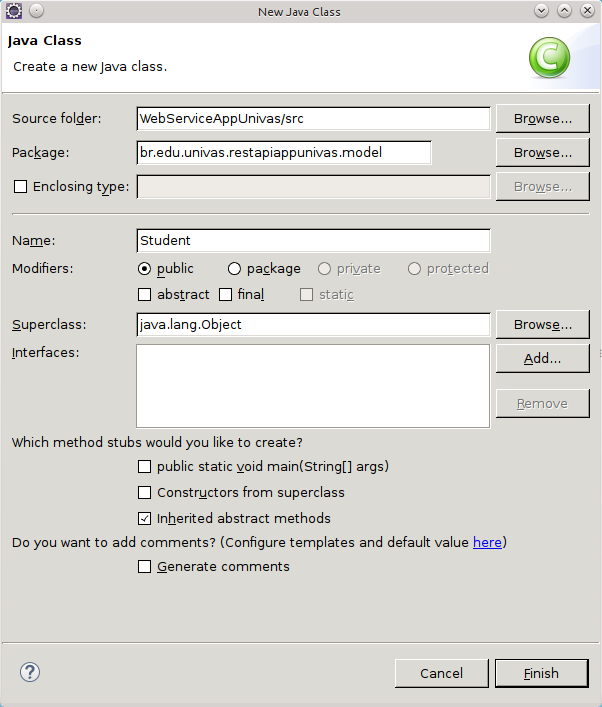
\includegraphics[scale=0.8]{./imagens/2_q_metodologico/4_procedimentos_resultados/43_webservice/432_desenvolvimento/desws10.png}}
		\caption[Sem legenda]{Sem legenda.
			\textbf{Fonte:}Elaborado pelos autores.}
		\label{fig:desws10}
	\end{figure}
	
	\pagebreak

	\par Esta classe foi definida para representar as informações referente aos
alunos. o código da classe pode ser visto na Figura \ref{fig:desws11}. 
	
	
	\begin{figure}[h!]
		\begin{lstlisting} [style=custom_Java]	
	package br.edu.univas.restapiappunivas.model;
	/**
	 *imports omitidos
	 */
	
	@Entity
	@Table(name = "student")
	public class Student {
	
		@Id
		@SequenceGenerator(name = "id_student", sequenceName = "seq_id_student",
			allocationSize = 1) 
		@GeneratedValue(generator = "id_student", strategy = GenerationType.IDENTITY)
		@Column(name = "id_student", nullable = false)
		private Long idStudent;
	
		@Column(name = "id_external", nullable = false)
		private Long idDatabaseExternal;
	
		@Column(length = 100, nullable = false)
		private String name;
	
		@Column(length = 100, nullable = false)
		private String email;
	
		@OneToMany(mappedBy="student", fetch = FetchType.EAGER)
		private List<Event> events;
	
		@OneToOne(optional = false, fetch = FetchType.LAZY)
		@JoinColumn(name = "id_user")
		private User user;
	
		/**
		 * Omitidos todos Getters e Setters
		 */
	
		@Override
		public int hashCode() {
			/**
			 * Omitido
			 */
		}
	
		@Override
		public boolean equals(Object obj) {
			/**
			 * Omitido
			 */
		}
	
	}
\end{lstlisting}
		\caption[Sem legenda]{Sem legenda.
			\textbf{Fonte:}Elaborado pelos autores.}
		\label{fig:desws11}
	\end{figure}
	
	\pagebreak
	
	\par É válido lembrar esta classe possui anotações para que possa ser
reconhecida como uma entidade do JPA, e assim persistida no banco de dados
quando necessário. Além disso estas anotações possuem outras finalidades
específicas. A seguir estão listadas todas as anotações  que foram usadas na
classe \texttt{Student.java} e nas outras classes que fazem parte do mapeamento
objeto relacional da aplicação.

	\begin{itemize}
	  \item \texttt{@Entity}: esta anotação foi necessária para que esta classe
	  pudesse ser reconhecida como uma entidade do JPA e assim persistida no banco
	  de dados;
	  \item \texttt{@Table}: anotação que possui algumas configurações relativas a
	  tabela no banco de dados, a qual esta entidade representa, no caso da classe'
	  mostrada anteriormente é configurado o nome da tabela;
	  \item \texttt{@Id}: esta anotação fica sobre o atributo que representa a
	  chave primária no banco de dados;
	  \item \texttt{@SequenceGenerator}: esta anotação define qual será o modo com
	  que a chave primaria será incrementada.
	  \item \texttt{@Column}: define algumas propriedades do campo da tabela do
	  banco de dados, o qual o atributo que ele anota representa. Estas
	  configuraçãoes podem são:
		  	\begin{itemize}
		    	\item \texttt{name}: muda o nome do campo;
		    	\item \texttt{length}: determina o tamanho em caracteres que o campo
		    	aceitará;
		    	\item \texttt{nullable}: define se o preenchimento do campo é obrigatório;
		    	\item \texttt{unique}: este atributo define se o campo aceitará valores
		    	únicos;
		    \end{itemize}
	  \item \texttt{@OneToMany}: representa um relacionamento um-para-muitos no
	  banco de dados. Anotam coleções de outras entidades;
	  \item \texttt{@ManyToOne}: representa um relacionamento
	  muitos-para-um no banco de dados. Este é a contraparte da anotação
	  um-para-muitos;
	  \item \texttt{@OneToOne}: representa um relacionamento um-para-um no banco de
	  dados.
\end{itemize}
 
	\par Esta classe faz parte do mecanismo de persistêcia de dados e é
simplesmente um  pojo ou seja, um objeto  simples que contêm somente atributos
privados e os métodos \textit{getters} e \textit{setters} que servem apenas
para encapsular estes atributos. Além desta classe, foram criadas outras com os
mesmos propósitos. Estas classes podem ser vistas na Figura \ref{fig:desws12}. 
	
	
	\begin{figure}[h!]
		\centerline{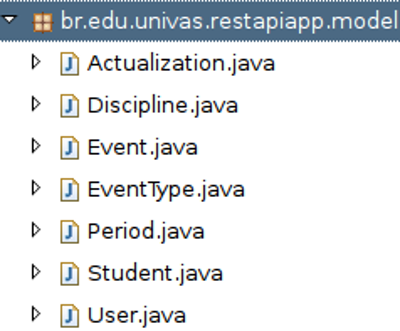
\includegraphics[scale=0.8]{./imagens/2_q_metodologico/4_procedimentos_resultados/43_webservice/432_desenvolvimento/desws12.png}}
		\caption[Sem legenda]{Sem legenda.
			\textbf{Fonte:}Elaborado pelos autores.}
		\label{fig:desws12}
	\end{figure}
	
	\pagebreak
	
	\par Estas classes tinham a mesma finalidade da anterior, porém com pequenas
diferenças no que diz respeito à atributos, metodos e anotações. Estas classes
representam, de maneira individual, as tabelas no banco de dados.

	%04 - HashCode e equals
	\par E por fim, para cada classe que representa uma entidade, foi necessário
implementar os métodos \texttt{hashCode} e \texttt{equals}, para que estas
pudessem facilmente ser comparadas e diferenciadas em relação aos seus
valores, haja visto que cada instância destas classes representa um registro
no banco de dados.
	
	%05 - Configuração do persistence.xml
	\par Em seguida à criação das entidades, foi necessário configurar o arquivo
\texttt{persistence.xml} que fica dentro do \textit{classpath} do projeto
Java ou seja, dentro da mesma pasta onde estão contidos pacotes do
projeto. Este arquivo é extremamente importante, pois é nele que estão todas
as configurações relativas à conexão com o banco de dados, configurações
referentes ao Dialeto SQL que vai ser usado para as consultas e configurações
referentes ao \textit{persistence unit} que é o conjunto de classes mapeadas
para o banco de dados.	O arquivo \texttt{persistence.xml} está exposto na
Figura \ref{fig:qm11}.

	\begin{figure}[h!]
		%persistence.xml
\begin{lstlisting} [style=custom_XML]
<?xml version="1.0" encoding="UTF-8"?>
<persistence version="2.1"
	xmlns="http://xmlns.jcp.org/xml/ns/persistence" 
	xmlns:xsi="http://www.w3.org/2001/XMLSchema-instance"
	xsi:schemaLocation="http://xmlns.jcp.org/xml/ns/persistence
	http://xmlns.jcp.org/xml/ns/persistence/persistence_2_1.xsd">
		<persistence-unit name="WsAppUnivas" transaction-type="RESOURCE_LOCAL">
					<provider>
						org.hibernate.jpa.HibernatePersistenceProvider
					</provider>
					<properties>
								<property name="javax.persistence.jdbc.url"
									value="jdbc:postgresql://localhost:5432/wsappunivas" />
								<property name="javax.persistence.jdbc.user" 
									value="postgres" />
								<property name="javax.persistence.jdbc.password" 
									value="omitido" />
								<property name="javax.persistence.jdbc.driver" 
									value="org.postgresql.Driver" />
								<property name="hibernate.dialect" 
									value="org.hibernate.dialect.PostgreSQLDialect" />
								<property name="hibernate.format_sql" 
									value="true" />
								<property name="hibernate.temp.use_jdbc_metadata_defaults"
									value="false" />
								<property name="hibernate.show_sql" 
									value="true" />
								<property name="hibernate.hbm2ddl.auto" 
									value="create" />
					</properties>
		</persistence-unit>
</persistence>
\end{lstlisting}
		\caption[Arquivo \texttt{persistence.xml}]{Arquivo \texttt{persistence.xml}.
		\textbf{Fonte:}Elaborado pelos autores.}
		\label{fig:qm11}
	\end{figure}
	
	%06 - Confecção JpaUtil.java
	\par Em seguida à confecção do \texttt{persistence.xml} foi criada a
classe \texttt{JpaUtil} que está representada na Figura \ref{fig:qm12}.
Esta classe é responsável por criar uma \texttt{EntityManagerFactory} que é
uma  fábrica de instâncias de \texttt{EntityManager} que nada mais é que um
\textit{persistence unit} ou unidade de persistência. Essa classe tem a
responsabilidade de prover um modo de comunicação entre a aplicação e o banco
de dados. No entanto a classe \texttt{JpaUtil} cria uma única instância de
\texttt{EntityManagerFactory}, que é responsável por disponibilizar e
gerenciar as instâncias de \texttt{EntityManager} de acordo com a necessidade
da aplicação.
	
	\pagebreak
	\begin{figure}[h!]
		%classe JpaUtil.java

\begin{lstlisting} [style=custom_Java] 	
package br.edu.univas.restapiappunivas.util;

import javax.persistence.EntityManager;
import javax.persistence.EntityManagerFactory;
import javax.persistence.Persistence;

public class JpaUtil {
	private static EntityManagerFactory factory;

	static {
		factory = Persistence.createEntityManagerFactory("WsAppUnivas");
	}

	public static EntityManager getEntityManager() {
		return factory.createEntityManager();
	}

	public static void close() {
		factory.close();
	}

}
	
\end{lstlisting}
		\caption[Classe \texttt{JpaUtil.java}]{Classe \texttt{JpaUtil.java}.
		\textbf{Fonte:}Elaborado pelos autores.}
		\label{fig:qm12}
	\end{figure}
		
	\par Em seguida à construção das classes que fazem a parte da persistência de
dados, foi desenvolvido a parte de disponibilização de serviços
RESTful, fazendo uso do \textit{framework} Jersey. Com isso
pode-se construir a classe que representa o primeiro serviço do
\textit{webservice}, que é a classe \texttt{Alunos}. Essa classe representa um
contexto REST, e portanto, dispõe de alguns recursos. Esses recursos fazem a
recuperação e a transmissão dos dados do \textit{web service} para o aplicativo
Android. Essa classe e seus respectivos métodos  estão representada na
Figura .
		
		\par O \textit{webservice} pode fazer a busca de alunos pelo \texttt{id}
passado ou retornar uma coleção de eventos vinculados a um alunos, dependendo
do recurso acessado. Os tipos de dados que o \textit{webservice} consome e
retorna é o JSON\footnote{JSON - Javascript Object Notation}. Não foi
necessário fazer nenhuma implementação adicional relativa a este formato, pois
o próprio \textit{framework} Jersey faz o tratamento e a conversão dos tipos de
entrada e saída de dados. No caso do saída de dados, faz a conversão de objetos 
Java para JSON. E no caso de entrada tranforma um JSON em objeto
Java já conhecido pelo \textit{web service}. Com isso concluiu-se o
desenvolvimento do \textit{web service} que fornece os dados para o aplicativo.

	%23 - Módulo que ira fazer a busca dos dados na base da instituição de ensino
	%24 - Falar que vai ser simulado
	\par Para que fosse possível transmitir dados para o aplicativo, era
necessário receber as informações do sistema acadêmico da referida instituição,
haja vista que o \textit{web service} é independente do mesmo. Para esse
propósito é necessário  contruir um módulo que faça a importação dos dados
necessários para a base de dados do \textit{web service}. 

	\par Este por sua vez terá a responsabilidade de fazer a importação dos dados
periodicamente, e ainda tratar os tipos de dados recebidos para tipos
aplicáveis ao banco de dados local. Além disso é preciso notificar o módulo
responsável por invocar o serviço Google Cloud Messaging para que os
dispositivos dos alunos aos quais houveram atualizações nos dados, fossem
notificados e fizessem acesso ao \textit{web service} para solicitar esses
dados atualizados.

	\par Os procedimentos acima citados foram os passos até agora realizados com o
propósito de se alcançar os resultados esperados para essa pesquisa.






%07 - Explicar anotações dos pojos
%08 - Finalizando camada de persistência
%09 - Camada de serviço
%10 - Classes que disponibilizam serviços anotações
%11 - Explicar as entities criadas para disponibilizar os dados
%12 - Ctrls que fazem a busca dos dados
%13 - Problema do erro 500
%14 - Provedor de arquivos e contexto
%15 - Em todos citar o pom.xml
%16 - Configuração do web.xml
%17 - Módulo de varredura de atualizações com timerTask
%18 - Módulo de alerta de provas agendas no dia da prova
%20 - Módulo para disparar as mensagens para o gcm
%21 - Serviço que faz o registro de sender_id
%22 - Mostrar a estrutura do empacotamento depois de finalizado
							%implantação
						%\subsubsection{Implantação}	
						%	%\subsubsection{Implantação}

\chapter{DISCUSSÃO DE RESULTADOS} 

	\par Este capítulo tem por finalidade descrever os resultados obtidos nesta
pesquisa através de uma explicação teórico-prática.

	\par O presente trabalho teve por objetivos desenvolver uma solução que
permitisse disponibilizar informações da Universidade do Vale do Sapucaí
através de serviços e a construção de um aplicativo que utilize o serviço
criado, permitindo aos seus alunos consultarem suas notas, faltas e provas
agendadas do semestre corrente através de seus dispositivos móveis com sistema
operacional Android.

	\par Entre os principais benefícios alcançados por esta pesquisa, pode-se
afirmar que o \textit{web service} criou uma estrutura para que a universidade
possa disponibilizar informações através de serviços. Neste trabalho, o
\textit{web service} disponibiliza via REST a consulta de notas, faltas e
provas agendadas. Uma documentação básica da API pode ser vista a seguir.

	\begin{tiny}
\begin{enumerate}
	\item \textbf{Contexto da Aplicação} -
	http://<enderecoDoServidor>/WebServiceAppUnivas/
		\begin{itemize}
			\item \textbf{Contextos internos}
				\begin{itemize}
					\item \textbf{students} - contexto relacionados aos dados dos alunos
							\begin{itemize}
								
								\item events - recurso referente aos dados sobre eventos relacionados a
								alunos;
									\begin{itemize}
									  \item \textbf{GET} - recebe como parâmetro a matrícula do aluno
									  através da url, e devolve um JSON, com todos os eventos do semestre corrente
									  relacionados ao aluno;\\ Ex.: 
									  http://<enderecoDoServidor>/WebServiceAppUnivas/students/events/98004095
									  \item \textbf{POST} - Não Implementado
									  \item \textbf{PUT} - Não Implementado
									  \item \textbf{DELETE} - Não Implementado
									\end{itemize}									
								\item disciplines - recurso referente aos dados sobre disciplinas de
								alunos;
									\begin{itemize}
									  \item \textbf{GET} - recebe como parâmetro a matrícula do aluno
									  através da url, e devolve um JSON, com todos os disciplinas do semestre
									  corrente relacionadas ao aluno;\\ Ex.: 
									  http://<enderecoDoServidor>/WebServiceAppUnivas/students/disciplines/98004095
									  \item \textbf{POST} - Não Implementado
									  \item \textbf{PUT} - Não Implementado
									  \item \textbf{DELETE} - Não Implementado
									\end{itemize}
							\end{itemize}
					\item \textbf{users} - contexto relacionados aos dados dos usuários
						\begin{itemize}
									  \item \textbf{GET} - Não Implementado
									  \item \textbf{POST} - Não Implementado
									  \item \textbf{PUT} - recebe um JSON com os dados dos usuário e
									  retorna um cabeçalho com o código de  \textit{status} 200;
									  \item \textbf{DELETE} - Não Implementado
									\end{itemize}
				\end{itemize}
		\end{itemize}
\end{enumerate}
\end{tiny}
	
	\par O aplicativo Android, consome o serviço do \textit{web service} e do GCM
trazendo as informações aos estudantes de forma hábil, além de ser mais cômodo
para o usuário, uma vez que ele recebe os dados onde quer que esteja, desde que
possua acesso à internet.

	\par Além do mais, o software notifica o discente no momento em que é lançado
um novo evento beneficiando-o, tendo em vista que ele não precisa ficar
verificando se a nota já foi postada pelo professor, pois o sistema se
encarrega de avisá-lo.

	\par Como o aplicativo foi desenvolvido para a plataforma Android, ele pode ser
instalado em dispositivos de diferentes fabricantes, evitando ficar preso a um
hardware específico.

	\par Durante o período de desenvolvimento, foram realizados vários testes
através do emulador Android, presente na IDE Android Studio e em um
\textit{smartphone} Samsung S{3} Mini. Notou-se aí, que no dispositivo real a
velocidade da execução do aplicativo é bem maior se comparada ao emulador.

	\par Como os testes foram realizados sempre nos mesmos modelos de dispositivos,
há a possibilidade de ocorrer alguns problemas em relação ao \textit{layout}
dependendo do tamanho da tela do equipamento, contudo o fator de lógica da
aplicação não será afetado.

	\par O aplicativo desenvolvido possui fácil usabilidade, evitando com que o
aluno fique perdido ao buscar alguma informação. Para a organização das opções
que o software oferece aos discentes, foi criado uma tela do tipo
\textit{Navigation Drawer Layout}, que de acordo com \citeonline{android2015},
é um painel que normalmente fica escondido e aparece quando clicado no ícone do
aplicativo no canto superior esquerdo, o qual contém os dados de navegação do
software semelhante a um menu. Na Figura \ref{fig:dr}, é ilustrado o painel de
navegação do aplicativo.
	 
\begin{figure}[h!]
	\centerline{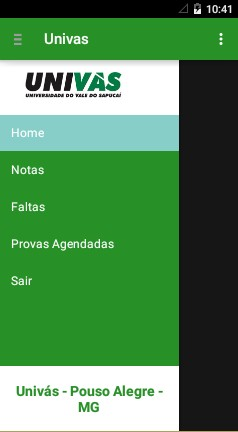
\includegraphics[scale=0.8]{./imagens/3_discussao_resultados/dr.jpg}}
	\caption[Tela principal do aplicativo com as opções de navegação]{Tela
	principal do aplicativo com as opções de navegação.
	\textbf{Fonte:}Elaborado pelos autores.}
	\label{fig:dr}
\end{figure}

	\par Para apresentar as informações, foi utilizado uma lista do tipo
\texttt{ExpandableListView} que segundo \citeonline{android3}, é um
\textit{widget} que exibe uma lista de itens e ao selecionar um desses
elementos, a tela é estendida apresentando os subitens da opção escolhida. Na
Figura \ref{fig:dr1} é mostrada a tela que lista as disciplinas sendo que
Tópicos Avançados está selecionada.


\begin{figure}[h!]
	\centerline{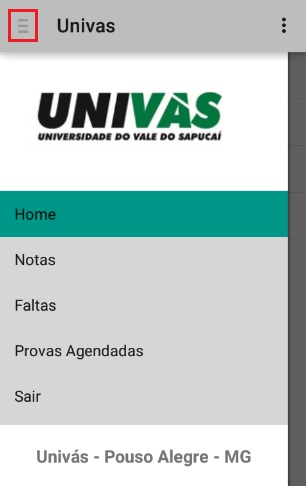
\includegraphics[scale=0.8]{./imagens/3_discussao_resultados/dr1.png}}
	\caption[Lista de disciplinas]{Lista de disciplinas.
		\textbf{Fonte:}Elaborado pelos autores.}
	\label{fig:dr1}
\end{figure}

	\pagebreak

	\par O GCM foi utilizado neste projeto para fazer a transmissão dos eventos do
servidor para o aplicativo. Com ele, a troca de dados tornou-se mais rápido e
simples, pois toda a lógica de entrega fica por conta da Google.

	\par Quando se trata de apenas uma informação para um único dispositivo, o
controle é simples, mas a partir do momento em que há vários equipamentos para
receber informações distintas, o gerenciamento torna-se mais complexo. Por
isso, pode-se afirmar que o GCM solucionou este problema, mostrando-se eficaz
na transmissão dos dados, além de ser de fácil configuração. A Figura
\ref{fig:dr2}, ilustra uma notificação logo após o GCM ter entregue uma
mensagem ao aplicativo. Ao baixar a paleta de notificação será apresentado um
resumo da notificação, como apresenta a Figura \ref{fig:dr3}.


\begin{figure}[h!]
	\centerline{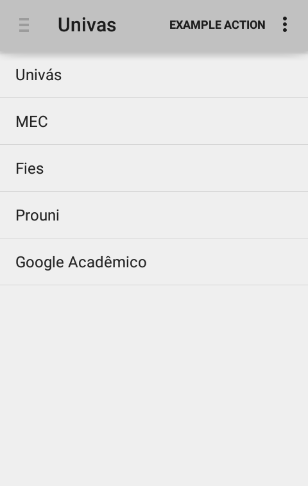
\includegraphics[scale=0.8]{./imagens/3_discussao_resultados/dr2.png}}
	\caption[Notificação na barra de notificações do dispositivo.]{Notificação na
	barra de notificações do dispositivo.
	\textbf{Fonte:}Elaborado pelos autores.}
	\label{fig:dr2}
\end{figure}


\begin{figure}[h!]
	\centerline{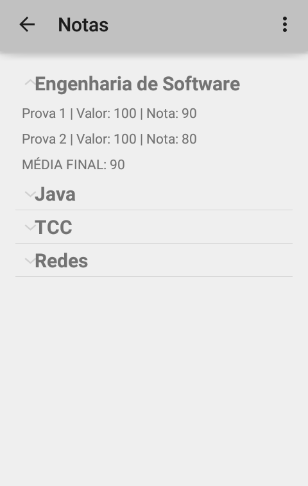
\includegraphics[scale=0.8]{./imagens/3_discussao_resultados/dr3.png}}
	\caption[Paleta de notificação estendida]{Paleta de notificação estendida.
		\textbf{Fonte:}Elaborado pelos autores.}
	\label{fig:dr3}
\end{figure}

\pagebreak

	\par Ao clicar na notificação é apresentado para o aluno a tela que exibe os
dados da notificação. Na Figura \ref{fig:dr4}, pode-se ver a tela exibindo as
informações de um evento de notas.

\begin{figure}[h!]
	\centerline{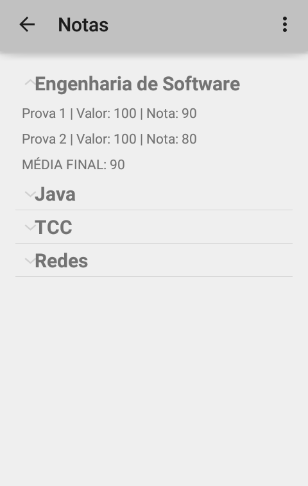
\includegraphics[scale=0.8]{./imagens/3_discussao_resultados/dr4.png}}
	\caption[Tela exibindo os dados após clicado na notificação]{Tela exibindo os
	dados após clicado na notificação.
	\textbf{Fonte:}Elaborado pelos autores.}
	\label{fig:dr4}
\end{figure}

	\par Portanto, sabendo-se que esta pesquisa enquadra-se no tipo de pesquisa
aplicada, o qual tem por finalidade desenvolver um produto real para resolver
um determinado problema e que a solução construída auxilia tanto a Univás, que
terá um nova forma de disponibilizar suas informações, quanto aos alunos, que
possuem a opção de consultarem suas informações acadêmicas através de
dispositivos móveis, entende-se que este trabalho atingiu suas expectativas.	

\chapter{CONCLUSÃO} 

	\par Com a realização desta pesquisa, constatou-se que no mercado mundial
existe um alto número de aparelhos celulares com sistema operacional Android,
pelos quais os usuários procuram soluções para suas as tarefas diárias. Assim, o
aplicativo desenvolvido neste trabalho, tem por finalidade informar ao
estudante suas notas, faltas e provas agendadas do semestre corrente. Além do
mais, no momento em que algum professor lançar eventos como notas, faltas ou
provas agendadas, o software envia uma notifica o aluno.

	\par O \textit{web service} criado, responde as requisições via REST oferecendo
a Univás uma oportunidade de disponibilizar suas informações através de
serviços. No presente momento, os serviços que são possíveis utilizar são a
consulta de notas, faltas e provas agendadas.

	\par As mensagens enviadas do servidor para o dispositivos móveis são
transmitidas também via REST através da API Google Cloud Messaging (GCM), da
Google, que oferece o recurso gratuitamente e que mostrou-se muito eficaz,
solucionando o problema do envio de notificações aos dispositivos dos alunos  e
de transmissão dos dados.

	\par Deve-se também destacar o grande número de materiais disponibilizados por
desenvolvedores e estudiosos da área, os quais possibilitaram aos autores desta
pesquisa o estudo e aprendizagem das teorias apresentadas nesta pesquisa, bem
como suas implementações.

	\par Portanto, apesar das dificuldades encontradas para a realização deste
trabalho, como realizar a comunicação entre o web service e o aplicativo
Android, percebeu-se que o software apresentado nesta pesquisa é de grande
utilidade aos alunos da Universidade do Vale do Sapucaí, pois conseguem
acompanhar seus desempenhos escolares através de seus equipamentos
\textit{mobile} e a Univás que tem agora, uma estrutura pronta para
disponibilizar suas informações através de serviços.

	\par Devido ao crescente número de dispositivos móveis é possível perceber uma
época favorável para explorar essas tecnologias. Sendo assim, este projeto
possibilita aos graduandos em Sistemas de Informação uma oportunidade para
acrescentar novas funcionalidades para esta aplicação em trabalhos futuros.

	\par Devido ao tempo escasso esse trabalho não trata a parte de segurança,
podendo ser implementado em outra oportunidade. São exibidas, apenas as
disciplinas do semestre corrente, sendo possível acrescentar a funcionalidade
para exibir todas as matérias já cursadas. Também pode-se criar o serviço para
que os alunos realizem a CPA, consultas de livros da biblioteca, permitir aos
professores lançarem notas no portal do aluno ou publicarem materiais, além de
possibilitar o acesso a outras plataformas como Windows Phone e IOS.

	\par Por fim, pode-se afirmar que o presente trabalho realizou seus objetivos,
os quais eram possibilitar aos alunos da Univás consultarem suas notas, faltas
e provas agendadas, notificando-os quando estes eventos ocorrem, além
desenvolver uma estrutura para a universidade poder disponibilizar informações
em forma de serviço, o que hoje ainda não acontece. Ainda, esta pesquisa foi de
grande relevância aos participantes do projeto, pois contribuiu por uma ampla
visão de resolução de problemas e um conhecimento vasto nas tecnologias
utilizadas.



\postextual %Início dos Elementos Pós-Textuais

%\citeoption{abnt-etal-cite=2}
%\citeoption{ABNT-final}

%\bibliography{nuapatex-options, biblio}			            % insere as REFERENCIAS
% (arquivo biblio.bib)
\bibliography{biblio}			            % insere as REFERENCIAS (arquivo
% biblio.bib)
\addcontentsline{toc}{chapter}{REFERÊNCIAS} % adiciona o título no sumário

\begin{apendicesenv}

%\apendicesname{APÊNDICES}
% Imprime uma página indicando o início dos apêndices
\partapendices*

\addcontentsline{toc}{chapter}{APÊNDICES}

\chapter*{Criação de um projeto Dynamic Web Project no Eclipse Luna}
\label{apendice:1}
\captionsetup[figure]{list=no}
	
	\par Para proceder com a criação de um projeto do tipo \textit{Dynamic Web
Project} no Eclipse, é necessário acessar na IDE, a opção \textbf{File -> New->
Dynamic Web Project} como pode ser visto na Figura \ref{fig:desws3}.

	
	\begin{figure}[h!]
		\centerline{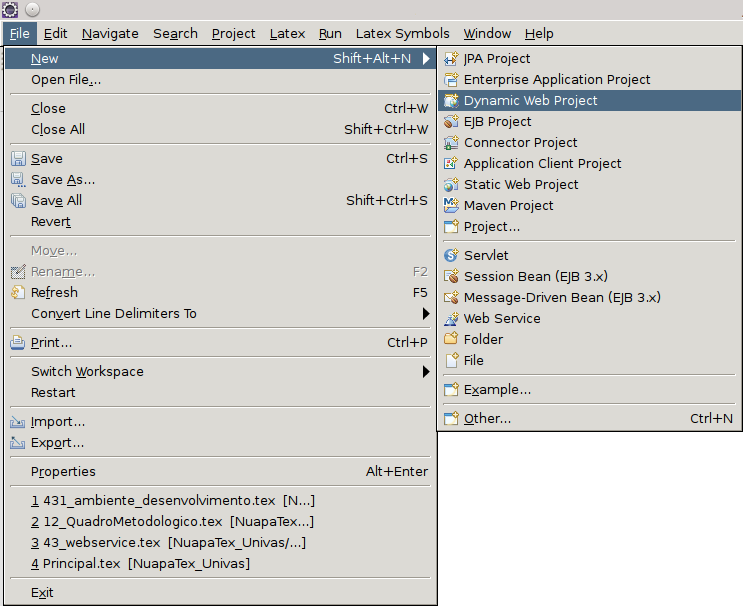
\includegraphics[scale=0.8]{./imagens/2_q_metodologico/4_procedimentos_resultados/43_webservice/432_desenvolvimento/desws3.png}}
		\caption[Tela \textit{New Database\ldots}]{Tela \textit{New Database\ldots}.
			\textbf{Fonte:}Elaborado pelos autores.}
		\label{fig:desws3}
	\end{figure}
	
	\pagebreak
	
 	\par Em seguida foi apresentada uma tela para o preenchimento de alguns dados
 requeridos para a criação do projeto. Destas informações somente foi preenchido
 o nome do projeto. As outras informações continuaram sendo as que vem por
 padrão da IDE. A janela apresentada e as informações preenchidas podem ser
 vistas na Figura \ref{fig:desws4}.

	\begin{figure}[h!]
		\centerline{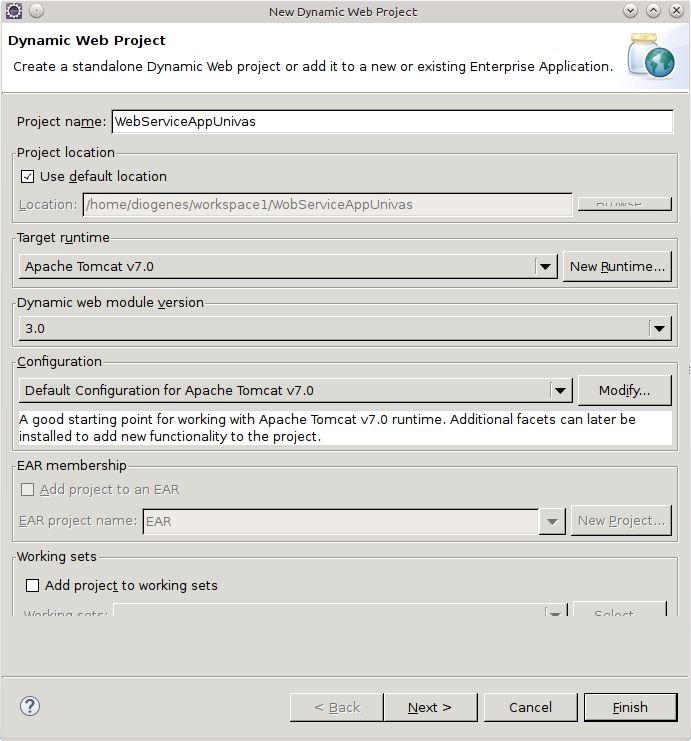
\includegraphics[scale=0.8]{./imagens/2_q_metodologico/4_procedimentos_resultados/43_webservice/432_desenvolvimento/desws4.png}}
		\caption[Tela para criação de um novo projeto no Eclipse]{Tela para criação de um novo projeto no Eclipse.
			\textbf{Fonte:}Elaborado pelos autores.}
		\label{fig:desws4}
	\end{figure}
	
	\pagebreak
	
	
	\par Na próxima janela apresentada, que têm por função configurar a pasta de
códigos do projeto manteve-se a configuração apresentada pela IDE, como mostra
a Figura \ref{fig:desws5}.

	\begin{figure}[h!]
		\centerline{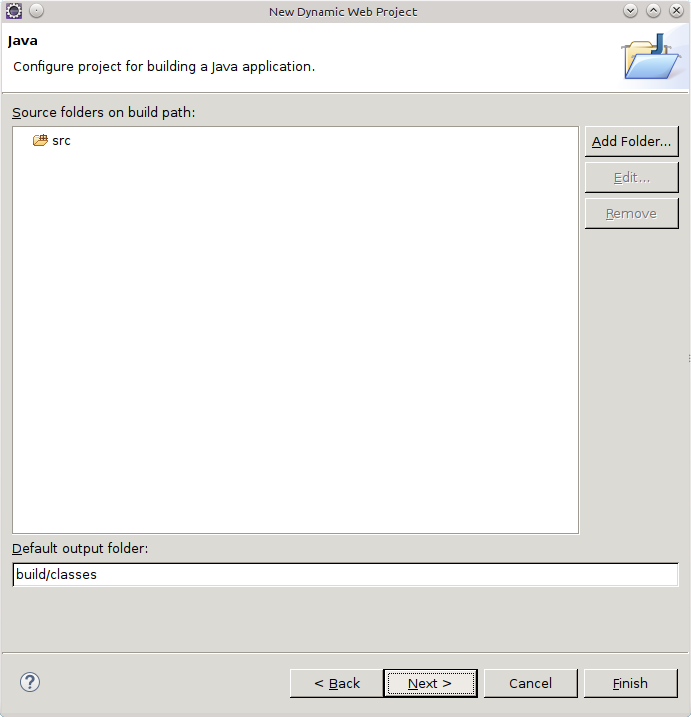
\includegraphics[scale=0.8]{./imagens/2_q_metodologico/4_procedimentos_resultados/43_webservice/432_desenvolvimento/desws5.png}}
		\caption[Tela para criação de um novo projeto no Eclipse]{Tela para criação de um novo projeto no Eclipse.
			\textbf{Fonte:}Elaborado pelos autores.}
		\label{fig:desws5}
	\end{figure}
	
	\pagebreak
	
	\par Na sequência, na tela que foi apresentada era necessário preencher o
campo \textbf{Context root} com o contexto principal da aplicação web que
acabou mantendo o próprio nome da aplicação. Além disso foi marcado a opção
\textbf{Generate web.xml deployment descriptor}, para que ao criar o projeto, a
própria IDE criasse o arquivo \texttt{web.xml}, arquivo responsável por algumas
configurações da aplicação web. Esta tela está apresentada na Figura
\ref{fig:desws6}.

	\begin{figure}[h!]
		\centerline{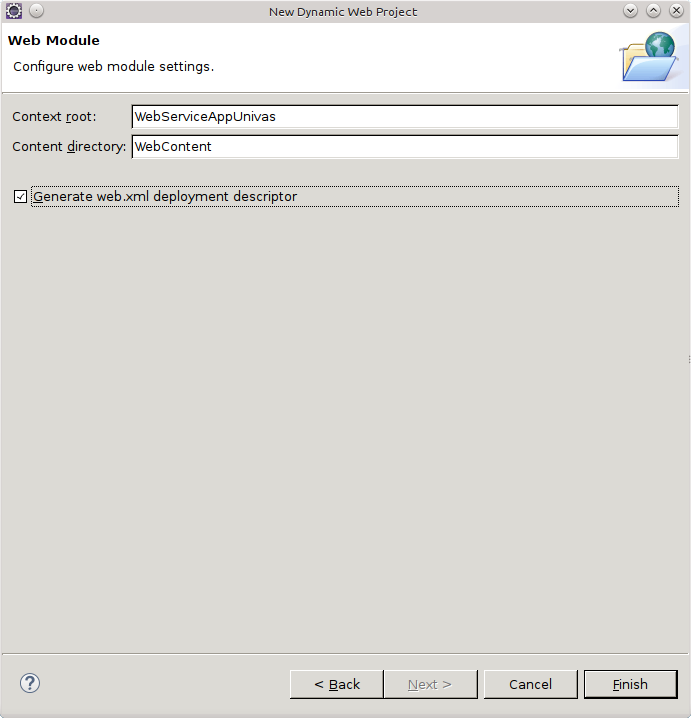
\includegraphics[scale=0.8]{./imagens/2_q_metodologico/4_procedimentos_resultados/43_webservice/432_desenvolvimento/desws6.png}}
		\caption[Tela para criação de um novo projeto no Eclipse]{Tela para criação de um novo projeto no Eclipse.
			\textbf{Fonte:}Elaborado pelos autores.}
		\label{fig:desws6}
	\end{figure}
	
	\pagebreak

	%03 - Mapeamento orm;	
		%	->Criação do pacote

	\par Após este passo foi concluído a criação do projeto.
	%, e já era possível iniciar os trabalhos com a camada de persistência de dados
	% do projeto.

%\chapter*{Título do Apêndice 2}



\end{apendicesenv}
%\begin{anexosenv}
	
	\partanexos*
	
	\addcontentsline{toc}{chapter}{ANEXOS}
	
	\chapter*{ANEXO I}


\end{anexosenv}

%

%\chapter*{ANEXO I}



\printindex

\end{document}